%! TEX program = xelatex
\documentclass[UTF8,a4paper,12pt,fontset=fandol]{ctexart}

\usepackage[top=2.5cm,bottom=2.5cm,left=2.5cm,right=2.5cm]{geometry}
\usepackage{amsmath,amssymb,bm}
\usepackage{booktabs,tabularx,multirow,longtable,array}
\usepackage{graphicx,float,subcaption}
\usepackage{enumitem}
\usepackage{xcolor}
\usepackage{listings}
\usepackage{url}
\usepackage[hidelinks]{hyperref}
\usepackage{appendix}

\graphicspath{{figures/}{figures/q1/}{figures/q2/}}
\setlength{\parindent}{2em}
\setlength{\parskip}{0pt}
\linespread{1.25}
\pagestyle{plain}

\ctexset{
  section={format=\zihao{4}\bfseries,beforeskip=1.2ex,afterskip=0.8ex},
  subsection={format=\zihao{-4}\bfseries,beforeskip=1ex,afterskip=0.6ex},
  subsubsection={format=\zihao{-4}\bfseries,beforeskip=0.8ex,afterskip=0.4ex}
}

\captionsetup{font=small,labelsep=quad}
\setlist{nosep,leftmargin=2em}

\lstset{
  basicstyle=\small\ttfamily,
  numbers=left,
  numberstyle=\tiny\color{gray},
  frame=single,
  breaklines=true,
  showstringspaces=false,
  keywordstyle=\color{blue!70!black},
  commentstyle=\color{green!45!black},
  stringstyle=\color{purple}
}

\begin{document}
\pagenumbering{arabic}
\setcounter{page}{1}

% ======================== 摘要专用页 ========================
\begin{center}
  {\zihao{3}\bfseries NIPT的时点选择与胎儿的异常判定}
\end{center}

\begin{center}
  {\zihao{4}\bfseries 摘\quad 要}
\end{center}

本文针对男胎Y染色体浓度的影响关系及不同BMI人群的NIPT检测时点选择开展建模分析。首先识别“孕妇---采血---重复测序”的层级结构，将1082条测序记录聚合为267名孕妇的1021次采血，并建立含随机截距、随机孕周斜率和孕周二次项的线性混合效应模型。结果表明，Y染色体浓度随孕周呈显著非线性上升趋势，BMI具有显著负向影响，年龄的独立效应不显著；未聚合数据的敏感性分析得到一致结论。

在此基础上，将Y染色体浓度不低于$4\%$定义为达标，比较线性、二次交互、样条Logistic及梯度提升树等候选模型。按孕妇分组的五折交叉验证和一标准误差规则最终选择线性Logistic模型，其LogLoss为0.3702，AUC为0.5862。随后利用CART将BMI划分为$B<28.63$、$[28.63,29.59)$、$[29.59,31.30)$、$[31.30,32.70)$及$B\geq32.70$五组，对应推荐检测时点为11.0、14.0、17.5、21.5和21.0周；最高BMI组采用达到$85\%$可靠性后先检并复测的策略。Bootstrap和测量误差扰动表明部分切点与时点仍具有不确定性，因此结果适合作为群体检测安排依据，不应替代个体临床诊断。

\vspace{0.8em}
\noindent\textbf{关键词：}无创产前检测；线性混合效应模型；Logistic回归；CART分组；敏感性分析

\newpage

% =========================== 正文 ===========================
\section{问题重述}

\subsection{问题背景}

无创产前检测（Non-invasive Prenatal Test，NIPT）是一种通过采集孕妇血液并分析其中胎儿游离DNA片段，对胎儿染色体异常风险进行评估的产前检测技术。与传统侵入性产前诊断方式相比，NIPT具有安全性较高、检测过程方便等特点，在唐氏综合征、爱德华氏综合征和帕陶氏综合征等常见染色体异常的早期筛查中具有重要作用。

NIPT检测结果的可靠性受到孕周、孕妇身体质量指数以及测序质量等多种因素影响。对于男胎，当Y染色体浓度达到一定水平时，检测结果才具有较高的可信度。若检测时间过早，胎儿游离DNA浓度可能不足，从而增加检测失败或结果不稳定的可能；若检测时间过晚，又可能缩短发现异常后的临床处理时间。因此，如何在检测可靠性与早期发现风险之间取得平衡，是NIPT时点选择中的重要问题。

此外，不同孕妇在年龄、身高、体重、BMI和妊娠状况等方面存在个体差异，采用统一的检测时间难以适用于所有人群。对于不携带Y染色体的女胎，还需要结合染色体Z值、GC含量和读段质量等信息建立异常判定方法。基于上述背景，本文利用给定的男胎与女胎NIPT检测数据，研究男胎检测时点的合理选择，并建立女胎染色体异常判定模型。

\subsection{问题要求}

针对附件所给出的男胎与女胎NIPT检测数据，本文需要完成以下四项任务：

\textbf{问题一：}分析男胎Y染色体浓度与孕妇检测孕周、BMI及其他相关指标之间的关系，建立相应的关系模型，并检验模型及相关变量的显著性。

\textbf{问题二：}在BMI是影响男胎Y染色体浓度最早达标时间主要因素的条件下，对男胎孕妇进行合理的BMI分组，给出各组BMI区间和最佳NIPT检测时点，使潜在风险尽量降低，并分析检测误差的影响。

\textbf{问题三：}在问题二基础上，进一步考虑年龄、身高、体重等个体因素，以及检测误差和Y染色体浓度达标比例的影响，重新确定合理的BMI分组和各组最佳NIPT检测时点。

\textbf{问题四：}针对女胎不携带Y染色体的特点，以附件AB列中的13、18、21号染色体非整倍体结果作为异常判定依据，综合考虑染色体Z值、GC含量、测序读段指标、相关比例、X染色体浓度和BMI等因素，建立女胎异常判定方法。

\section{问题分析}

\subsection{问题一分析}

问题一研究男胎Y染色体浓度与检测孕周、BMI及其他指标之间的数量关系，是后续确定最佳检测时点的基础。首先统一孕周表示方式并进行描述性统计和可视化，再建立Y染色体浓度与各影响因素之间的关系模型，通过参数显著性、拟合优度和残差分析评价模型。由于同一孕妇可能存在多次检测记录，还需处理个体内相关性，预期得到孕周、BMI等因素的影响方向、影响程度及统计显著性。

\subsection{问题二分析}

问题二承接问题一，将研究目标由“解释Y染色体浓度的变化”转化为“确定不同BMI人群的最佳NIPT检测时点”。利用问题一中孕周、BMI与Y染色体浓度之间的关系，将Y染色体浓度达到或超过$4\%$定义为达标，估计不同BMI和孕周下的达标概率。在此基础上对BMI进行数据驱动分组，并在检测可靠性与延迟发现风险之间进行权衡，为每组选择尽可能早且可靠的检测时点。最后通过重复测序、Bootstrap和误差扰动分析结论的稳定性。

\subsection{问题三分析}

问题三是对问题二的扩展。问题二主要依据BMI进行群体分组，但实际达标时间还可能受到年龄、身高、体重、妊娠方式和测序质量的影响。因此需在保留BMI分组这一实际应用形式的同时，建立多因素达标概率模型，将更多个体特征纳入组内风险计算，重新确定各组最佳检测时点，并检验误差条件下分组边界和推荐时点的稳定性。

\subsection{问题四分析}

问题四的研究对象由男胎转为女胎。本文将附件AB列为空定义为无异常，出现T13、T18、T21或其组合定义为异常；以各染色体Z值、X染色体浓度、GC含量、测序读段指标、BMI和孕周等作为候选特征建立分类模型。训练集和测试集按孕妇代码划分，避免重复记录造成信息泄漏，并使用召回率、特异度、F1值和ROC--AUC等指标评价女胎异常判定效果。

\section{模型假设}

\begin{enumerate}
  \item 假设附件中的检测记录及字段含义真实可靠，清洗过程中仅对同次采血的重复测序进行合并，不改变原始生物学观测。
  \item 假设同次采血的Y染色体浓度测量误差相互独立、均值为零，且其方差在研究范围内近似稳定，以便利用重复测序差异估计测量误差。
  \item 假设在$10$至$25$孕周的研究区间内，同一BMI水平下的群体达标概率不会随孕周增加而下降；观测中的局部波动主要由测量误差和个体差异造成。
  \item 问题二以首次检测时BMI作为基线BMI，并假设其能够代表孕妇所属的BMI群体，避免使用达标后的BMI造成时间信息倒置。
  \item 假设样本所代表地区的检测流程在研究期内保持一致，模型结论主要用于相似高BMI人群的群体时点建议，不直接替代个体临床诊断。
\end{enumerate}

\section{数据预处理}

\subsection{分析单位与重复测序合并}

男胎原始工作表包含1082条测序记录和267名孕妇。数据中既有同一孕妇的多次采血，也有同次采血的重复测序；部分重复结果虽然报告日期相差数日，但孕妇代码、检测抽血次数和记录孕周均相同。为避免将延后报告的技术复测误认为新的生物样本，本文统一以“孕妇代码、检测抽血次数”识别一次采血，对该次采血的Y染色体浓度、孕周、BMI和年龄取均值，并保留浓度最小值、最大值和测序次数用于误差分析。共识别40组同次采血重复测序，合并后得到1021次采血观测。

\begin{table}[H]
  \centering
  \caption{问题一、问题二统一的数据清洗统计}
  \label{tab:male-clean-summary}
  \begin{tabular}{cc}
    \toprule
    项目 & 数量 \\
    \midrule
    原始检测记录 & 1082条 \\
    男胎孕妇 & 267人 \\
    聚合后采血观测 & 1021次 \\
    同次采血重复测序组 & 40组 \\
    \bottomrule
  \end{tabular}
\end{table}

\subsection{变量标准化与达标状态构造}

将“$a\mathrm{w}+b$”形式的孕周转换为连续周数：

\begin{equation}
  W=a+\frac{b}{7}.
  \label{eq:week-convert}
\end{equation}

利用体重除以身高平方复核BMI，差异均小于0.02。问题一使用各次采血记录对应的BMI解释连续Y染色体浓度；为避免把达标之后发生的体重变化反向用于预测，问题二采用每名孕妇首次检测时的BMI作为基线BMI。定义第$i$名孕妇第$j$次采血的达标状态为

\begin{equation}
  D_{ij}=\mathbb{I}\!\left(Y_{ij}\geq 0.04\right),
  \label{eq:q2-status}
\end{equation}

其中$Y_{ij}$表示Y染色体浓度。GC含量略低于$40\%$的记录仅设置质量标记而不机械删除，避免一次性剔除大量临界样本。

\subsection{删失结构说明}

267名孕妇中，217人在第一次检测时已经达标，只能确定真实达标时间早于首次检测，属于左删失；43人的真实达标时刻位于相邻两次检测之间，属于区间删失；7人在最后一次检测时仍未达标，属于右删失。因此，首次观测到达标的孕周不能直接等同于精确的生理达标时间，后续模型应尽量使用全部纵向检测记录。

\section{问题一的模型建立与求解}

\subsection{数据层级与分析单位}

男胎数据具有“孕妇---采血---重复测序”的三级结构：同一孕妇可能在多个孕周接受采血，同一次采血又可能被重复测序。因此，若直接将1082条测序记录视为相互独立的样本，会同时忽略孕妇内相关性并放大技术重复的权重。

本文将一次采血作为主分析单位。对具有相同孕妇代码和检测抽血次数的记录，将Y染色体浓度、孕周、BMI和年龄取均值，得到1021次采血观测，涉及267名孕妇；原始1082条记录仅用于敏感性分析。数据结构汇总见表~\ref{tab:q1-data-summary}。

\begin{table}[H]
  \centering
  \caption{问题一数据结构与分析单位}
  \label{tab:q1-data-summary}
  \begin{tabular}{lc}
    \toprule
    项目 & 数量 \\
    \midrule
    原始测序记录 & 1082条 \\
    男胎孕妇 & 267人 \\
    同次采血重复测序组 & 40组 \\
    聚合后采血观测 & 1021次 \\
    至少具有两个不同孕周观测的孕妇 & 260人 \\
    \bottomrule
  \end{tabular}
\end{table}

\subsection{探索性分析与变量筛选}

\subsubsection{Y染色体浓度与孕周、BMI的边际关系}

分别计算Pearson线性相关系数和Spearman秩相关系数，结果见表~\ref{tab:q1-correlation}。Y染色体浓度与孕周呈弱正相关，与BMI呈弱负相关。图~\ref{fig:q1-eda}中的LOWESS曲线与线性拟合存在明显差异，说明孕周效应可能包含非线性结构，BMI的方向则需要在控制孕周和个体差异后进一步检验。

\begin{table}[H]
  \centering
  \caption{Y染色体浓度与主要变量的边际相关性}
  \label{tab:q1-correlation}
  \begin{tabular}{lccc}
    \toprule
    变量 & Pearson相关系数 & Spearman相关系数 & 初步方向 \\
    \midrule
    检测孕周 & 0.1266 & 0.0843 & 正向 \\
    孕妇BMI & -0.1513 & -0.1550 & 负向 \\
    \bottomrule
  \end{tabular}
\end{table}

\begin{figure}[H]
  \centering
  \begin{subfigure}[t]{0.49\textwidth}
    \centering
    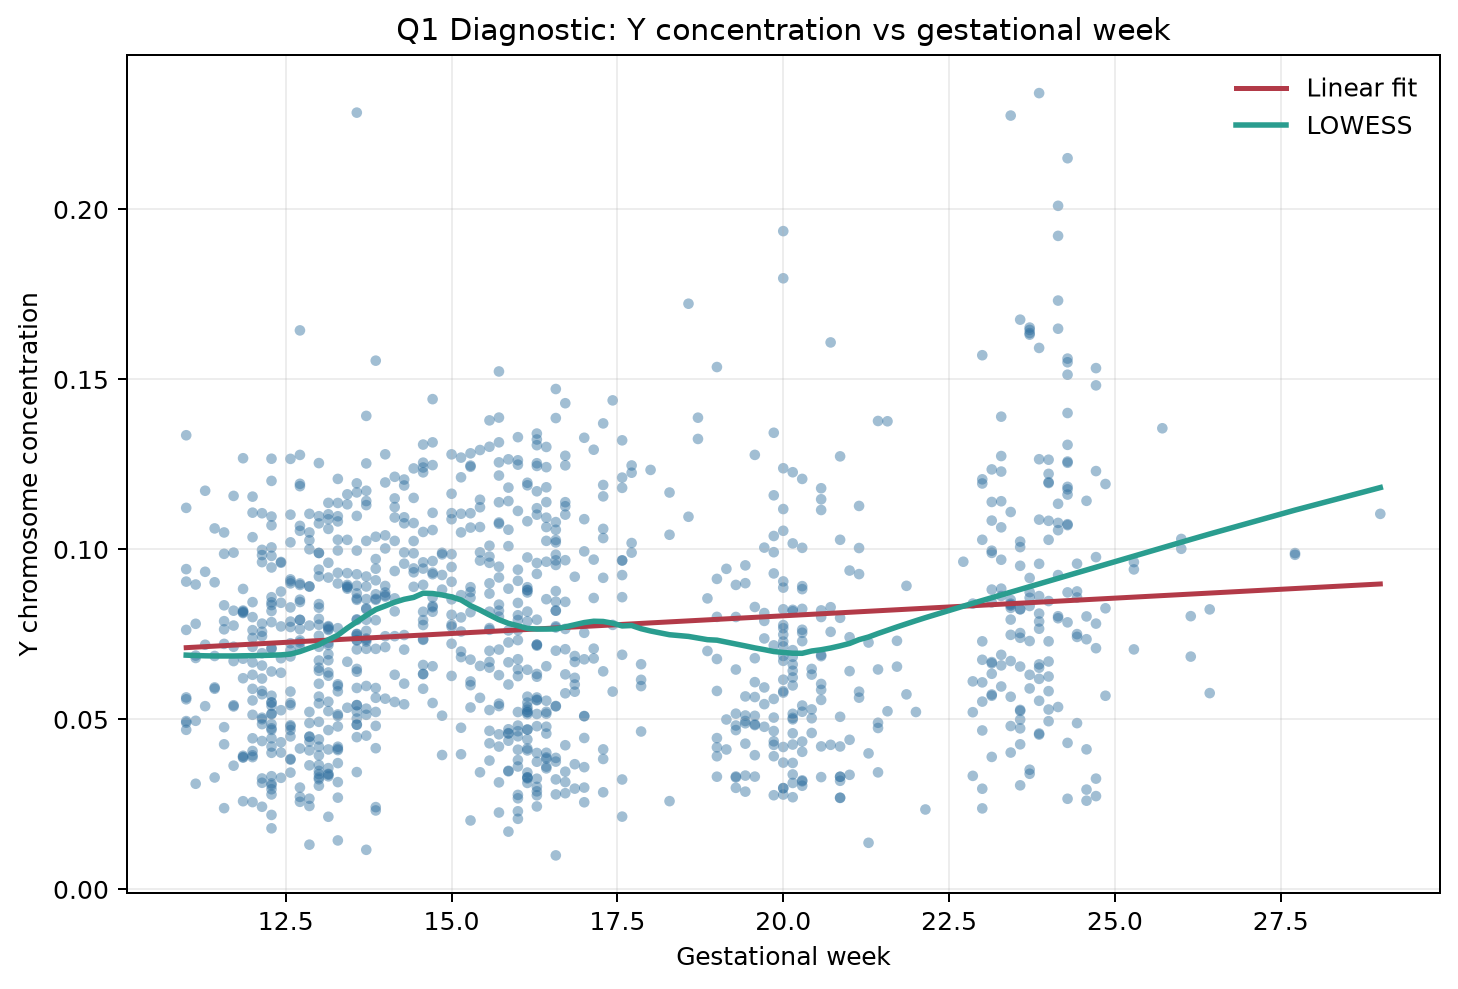
\includegraphics[width=\textwidth]{q1_y_vs_week.png}
    \caption{Y染色体浓度与检测孕周}
  \end{subfigure}
  \hfill
  \begin{subfigure}[t]{0.49\textwidth}
    \centering
    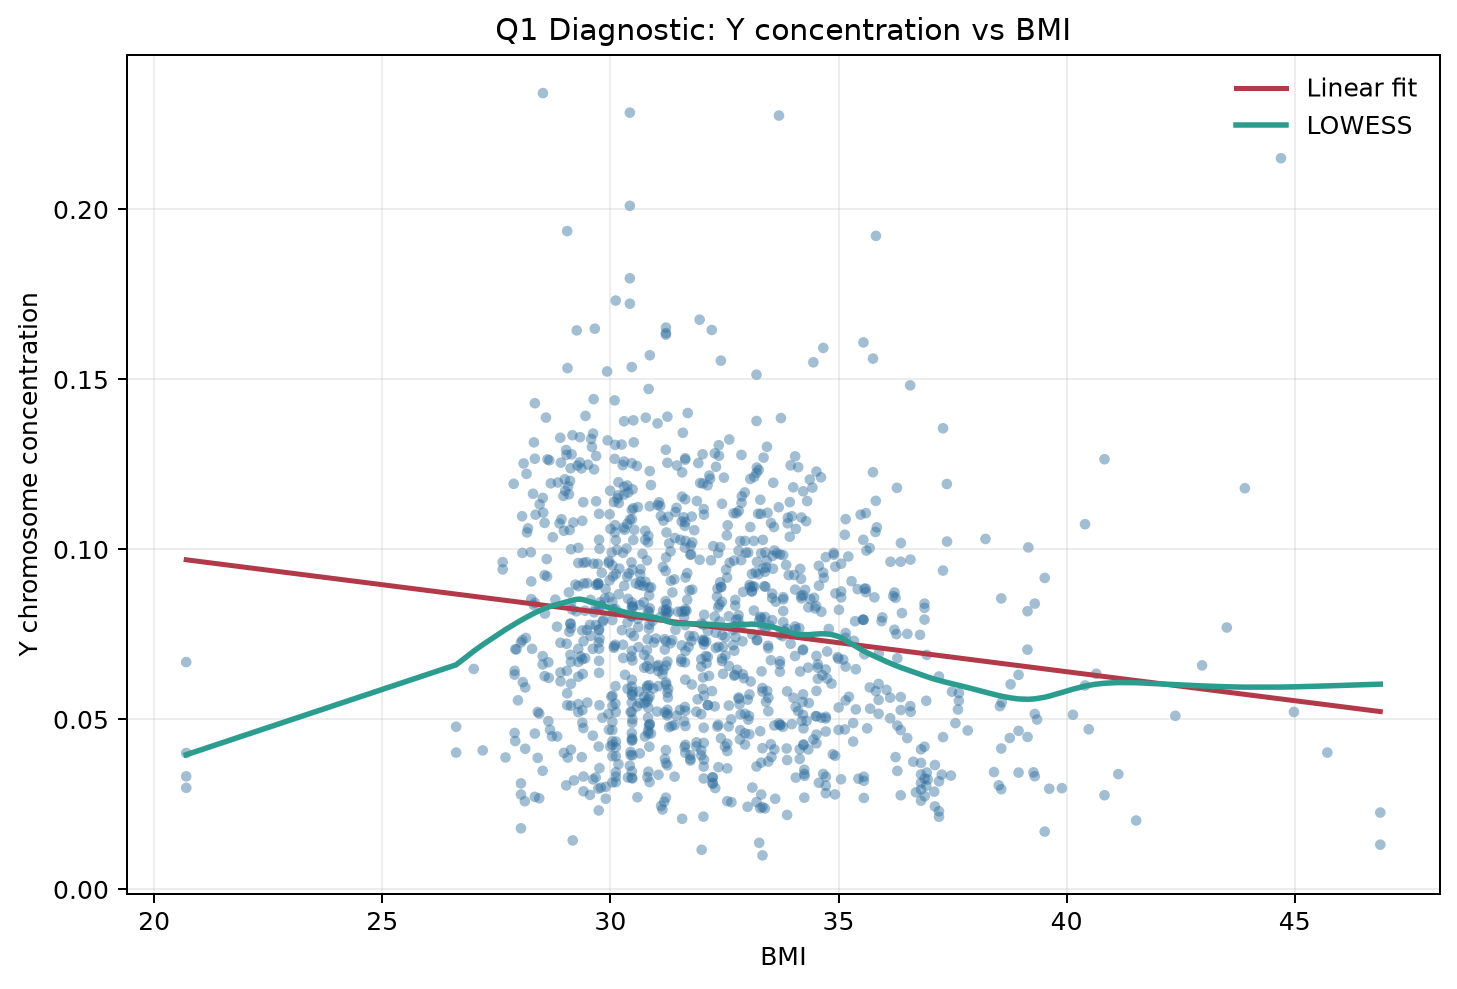
\includegraphics[width=\textwidth]{q1_y_vs_bmi.png}
    \caption{Y染色体浓度与孕妇BMI}
  \end{subfigure}
  \caption{Y染色体浓度与主要解释变量的散点图及平滑趋势}
  \label{fig:q1-eda}
\end{figure}

\subsubsection{重复测量与个体异质性}

图~\ref{fig:q1-trajectories}连接了同一孕妇在不同孕周的观测。不同孕妇的基础Y染色体浓度和随孕周变化的速度均存在明显差异，同一孕妇内部观测也并非独立。这表明普通多元线性回归的独立性假设不适合作为主模型，应使用能够显式描述孕妇内相关性的混合效应模型\cite{laird1982random,bates2015fitting}。

\begin{figure}[H]
  \centering
  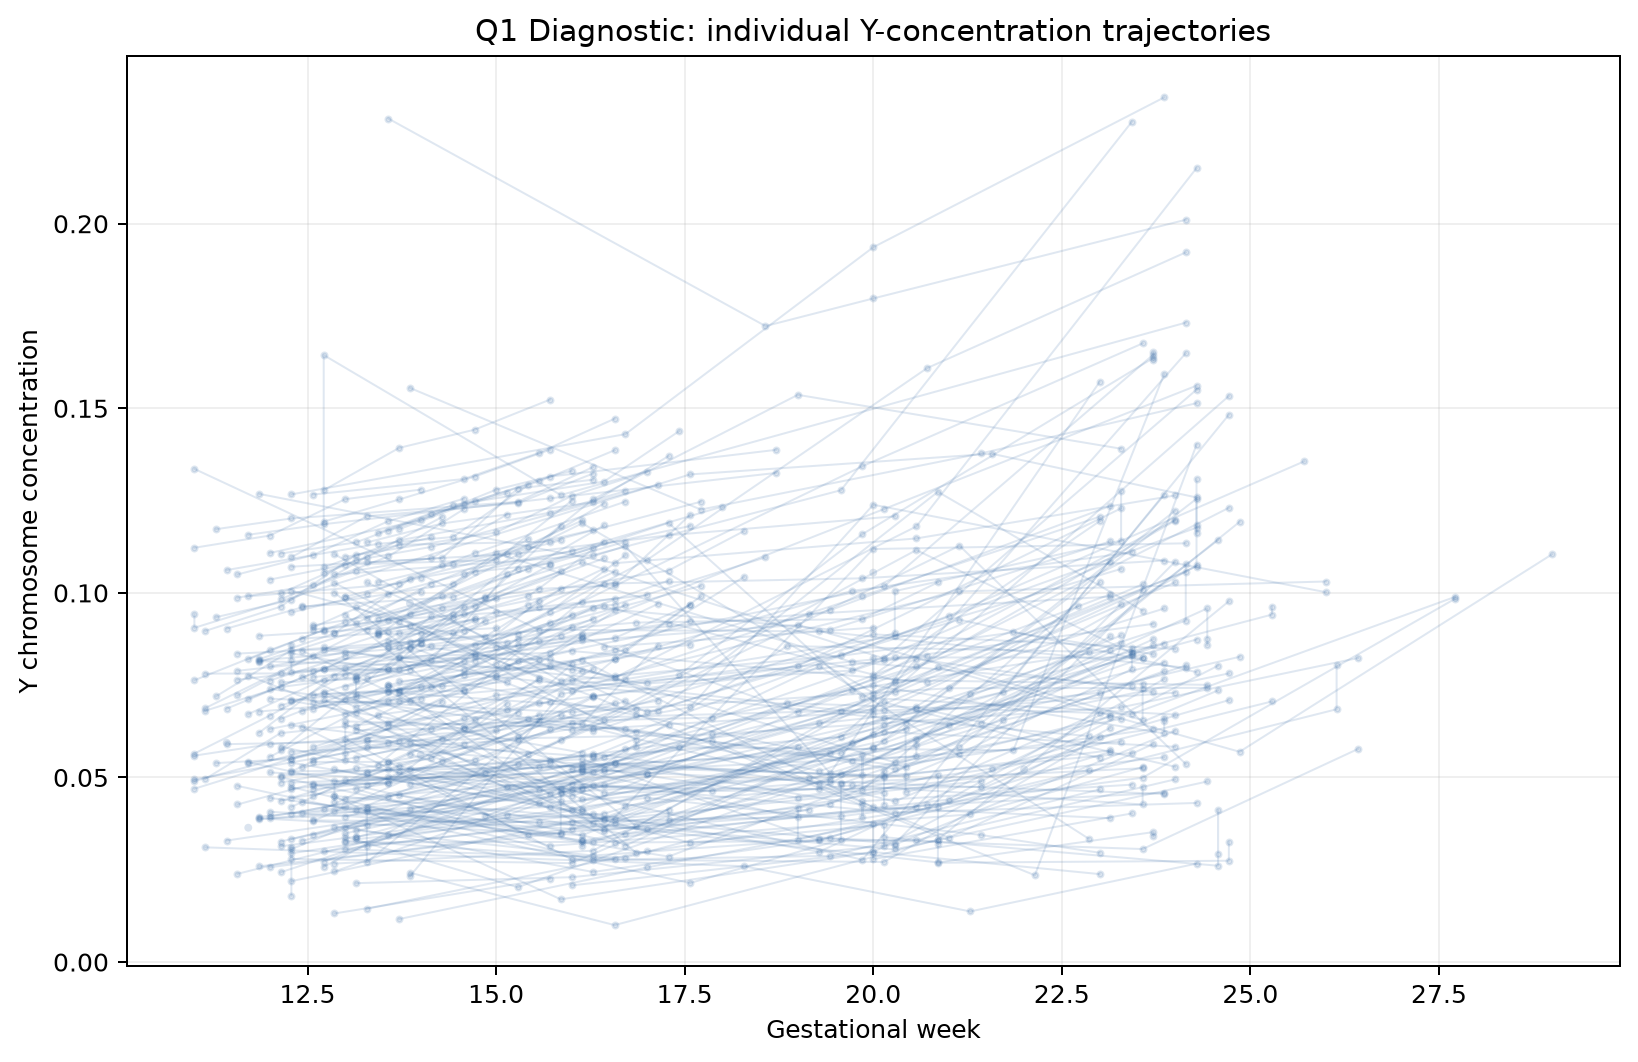
\includegraphics[width=0.93\textwidth]{q1_individual_trajectories.png}
  \caption{男胎孕妇Y染色体浓度的个体纵向轨迹}
  \label{fig:q1-trajectories}
\end{figure}

此外，BMI、体重和身高之间存在确定性关系，三者同时进入模型时VIF分别达到218.60、351.34和106.90，产生严重多重共线性。考虑到BMI是问题二、问题三的核心分组指标，最终保留BMI，不再同时加入体重和身高；年龄VIF为1.01，作为临床控制变量保留。

\subsection{线性混合效应模型}

\subsubsection{模型设定}

将第$i$名孕妇第$j$次采血的连续孕周记为$T_{ij}$，定义中心化孕周

\begin{equation}
  W_{ij}=T_{ij}-\bar T,\qquad \bar T=16.667343.
  \label{eq:q1-centered-week}
\end{equation}

以Y染色体浓度$Y_{ij}$为因变量，建立含随机截距与随机孕周斜率的线性混合效应模型：

\begin{equation}
  Y_{ij}=\beta_0+\beta_1W_{ij}+\beta_2W_{ij}^{2}
  +\beta_3B_{ij}+\beta_4A_i+b_{0i}+b_{1i}W_{ij}+\varepsilon_{ij},
  \label{eq:q1-lmm}
\end{equation}

其中，$B_{ij}$为BMI，$A_i$为年龄；$b_{0i}$和$b_{1i}$分别表示孕妇层面的随机截距与随机孕周斜率，刻画个体基础水平和变化速度的差异；$\varepsilon_{ij}$为采血层面的随机误差。固定效应和随机效应均采用最大似然法估计。

候选模型比较显示，仅包含孕周线性项的随机斜率模型AIC约为$-4855.4$；加入孕周二次项后AIC下降至$-4909.3$，且二次项显著。继续加入BMI二次项带来的改善很小，BIC反而略差。因此最终保留孕周二次项，BMI保持线性形式。

\subsubsection{固定效应估计与显著性检验}

最终模型固定效应结果见表~\ref{tab:q1-fixed-effects}。

\begin{table}[H]
  \centering
  \small
  \caption{问题一线性混合效应模型的固定效应估计}
  \label{tab:q1-fixed-effects}
  \begin{tabular}{lrrrr}
    \toprule
    变量 & 系数 & 标准误 & 95\%置信区间 & $p$值 \\
    \midrule
    截距 & 0.138148 & 0.022057 & $[0.094917,\ 0.181379]$ & $<0.001$ \\
    中心化孕周 & 0.003176 & 0.000253 & $[0.002680,\ 0.003673]$ & $<0.001$ \\
    中心化孕周平方 & 0.000264 & 0.000034 & $[0.000197,\ 0.000331]$ & $<0.001$ \\
    BMI & -0.001486 & 0.000524 & $[-0.002512,\ -0.000459]$ & 0.0046 \\
    年龄 & -0.000515 & 0.000487 & $[-0.001469,\ 0.000440]$ & 0.2908 \\
    \bottomrule
  \end{tabular}
\end{table}

孕周一次项和二次项均显著，说明Y染色体浓度与孕周之间存在显著非线性关系；结合图~\ref{fig:q1-fixed-prediction}可知，在样本主要观测范围内，Y染色体浓度总体随孕周增加而升高。BMI系数为$-0.001486$，在控制孕周、年龄和孕妇个体差异后仍显著，表示BMI每增加$1\ \mathrm{kg/m^2}$，模型预测的Y染色体浓度平均下降约0.001486，即0.149个百分点。年龄的$p=0.2908$，当前数据不足以证明其具有显著独立效应，但不能据此断言年龄完全没有影响。

\begin{figure}[H]
  \centering
  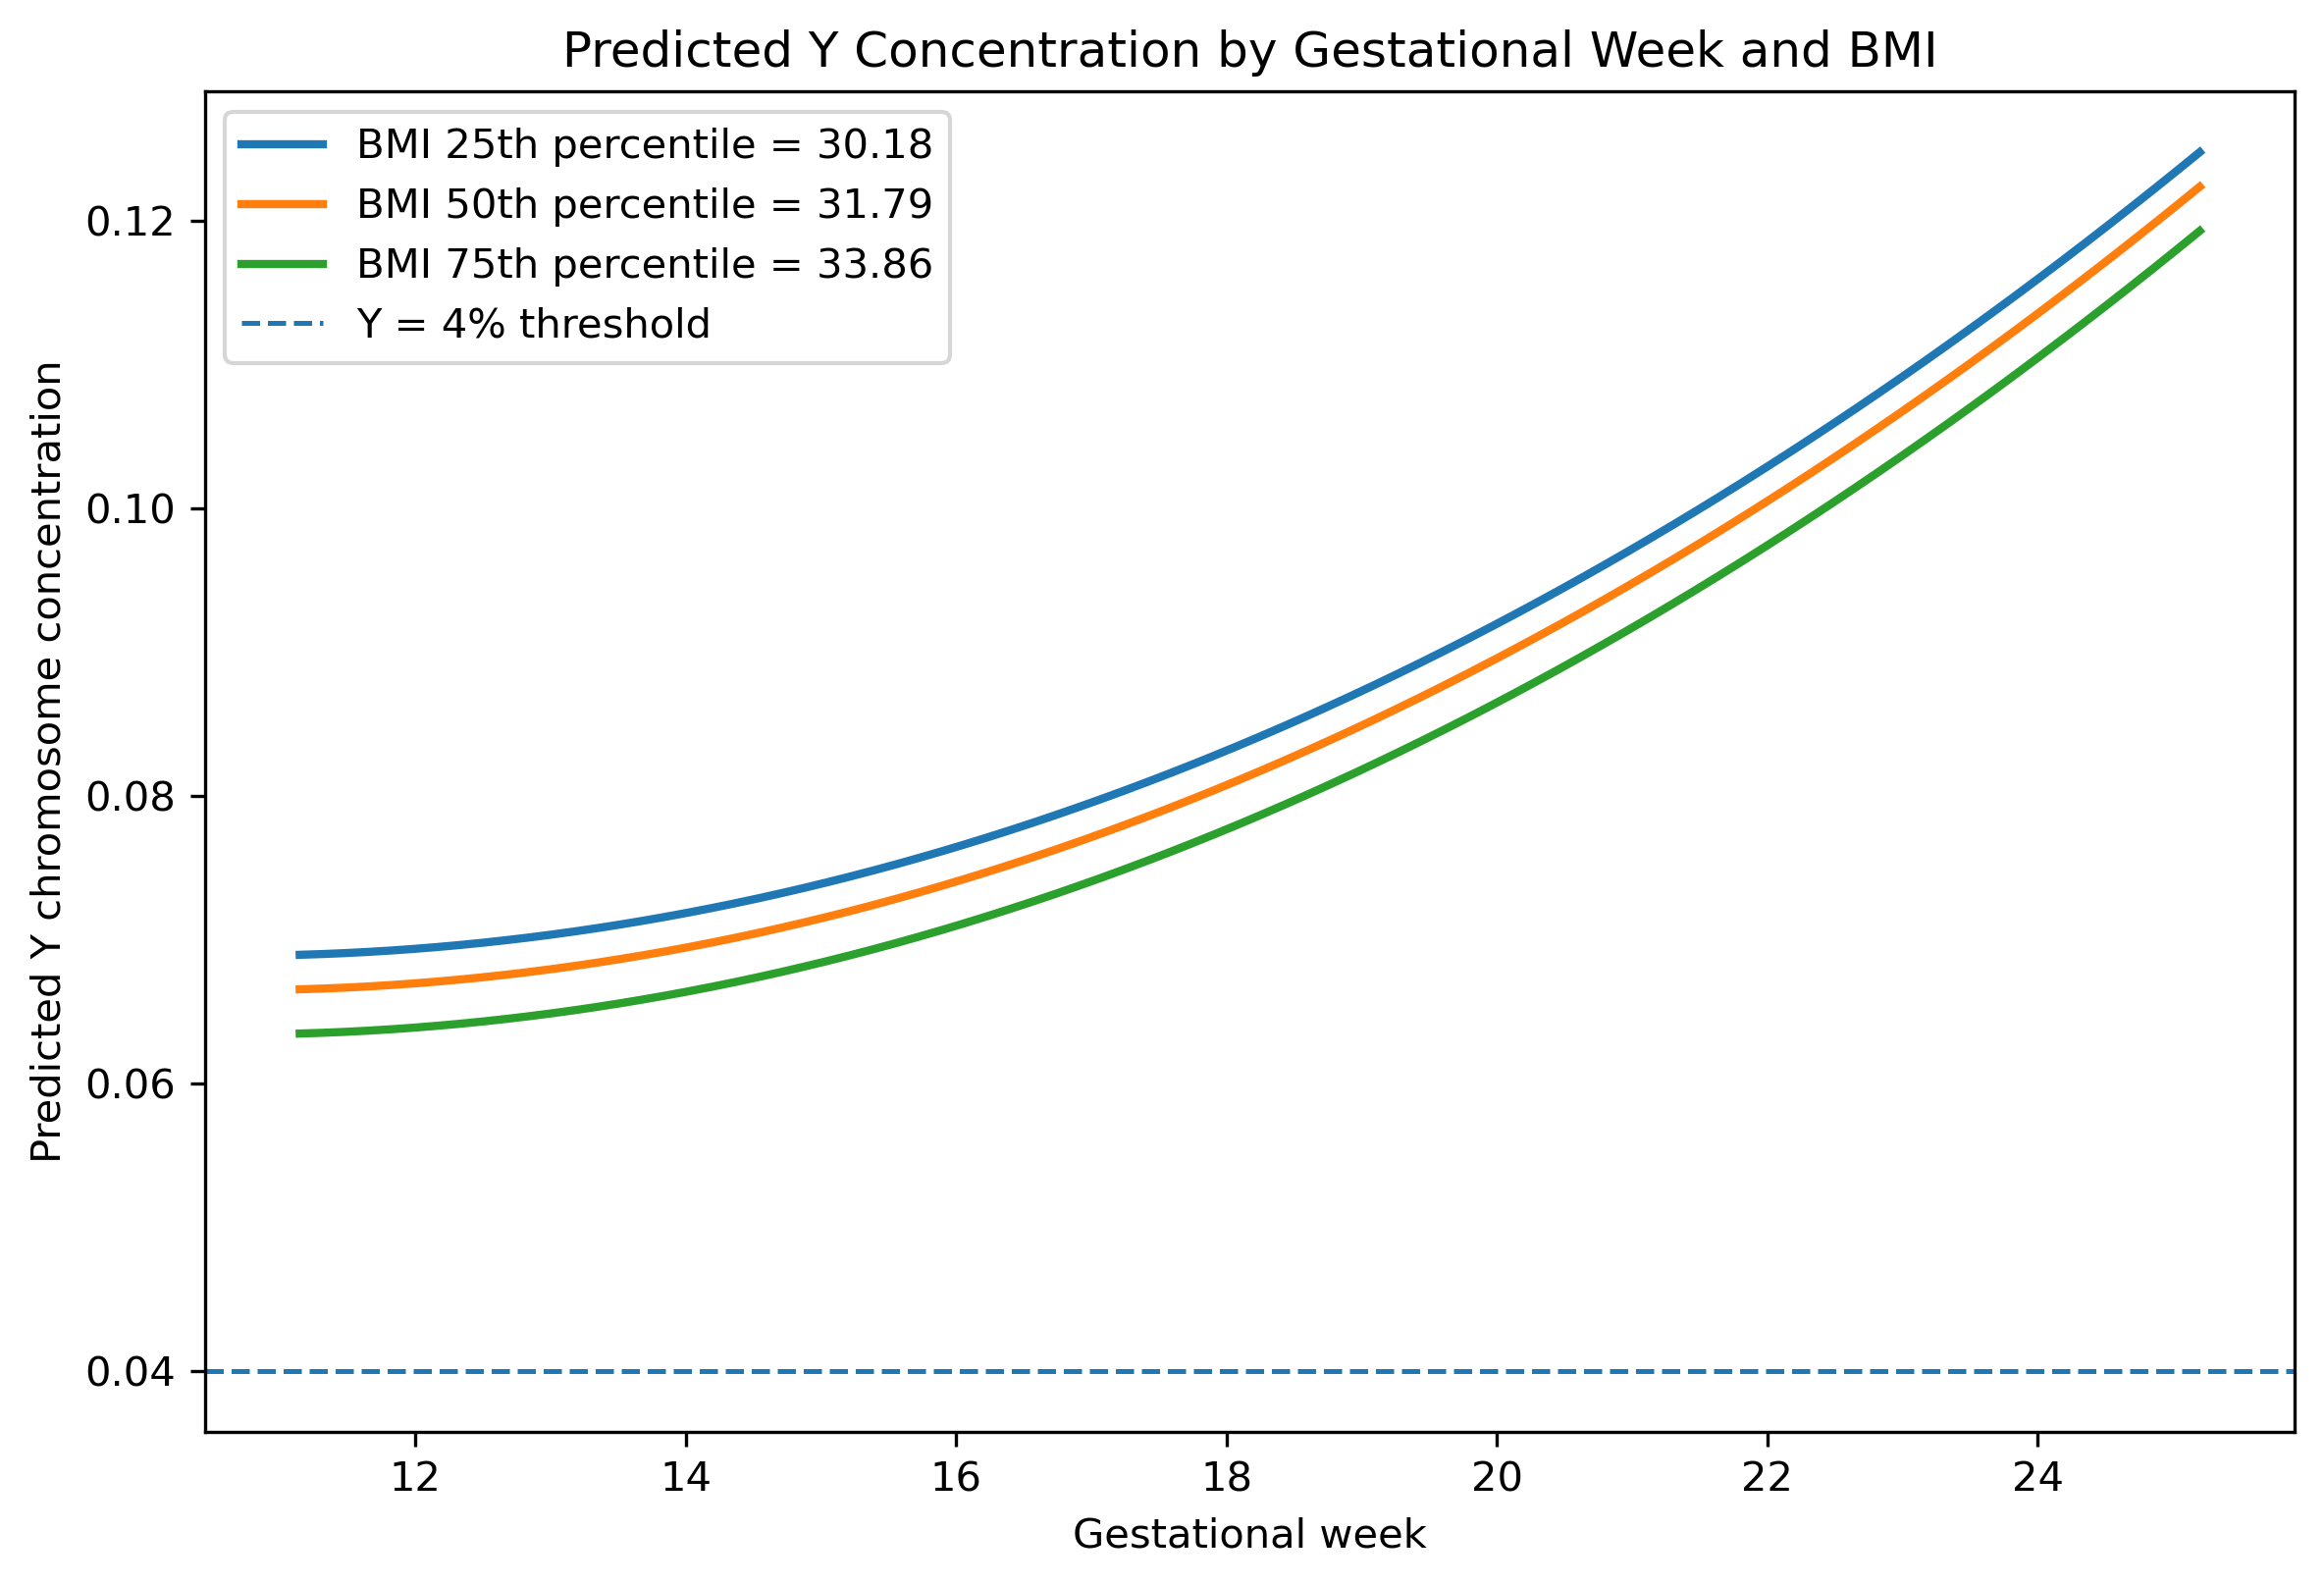
\includegraphics[width=0.88\textwidth]{q1_predicted_Y_by_week_BMI.png}
  \caption{不同BMI水平下Y染色体浓度随孕周变化的固定效应预测}
  \label{fig:q1-fixed-prediction}
\end{figure}

\subsubsection{随机效应与模型拟合}

模型共使用1021次采血和267名孕妇，已正常收敛，对数似然为2463.64，AIC为$-4909.29$，BIC为$-4864.93$。随机效应和残差估计见表~\ref{tab:q1-random-effects}。

\begin{table}[H]
  \centering
  \caption{问题一模型的随机效应与拟合指标}
  \label{tab:q1-random-effects}
  \begin{tabular}{lc@{\qquad}lc}
    \toprule
    指标 & 数值 & 指标 & 数值 \\
    \midrule
    随机截距标准差 & 0.030055 & 随机孕周斜率标准差 & 0.002725 \\
    截距--斜率相关系数 & 0.4851 & 残差标准差 & 0.013262 \\
    对数似然 & 2463.64 & AIC & $-4909.29$ \\
    观测数 & 1021 & 孕妇数 & 267 \\
    \bottomrule
  \end{tabular}
\end{table}

随机截距和随机斜率均具有不可忽略的变异，说明不同孕妇不仅基础Y染色体浓度不同，其随孕周变化的速度也存在差异，进一步支持使用随机截距与随机斜率模型。

\subsection{模型诊断与稳健性分析}

残差--拟合图和Q--Q图见图~\ref{fig:q1-diagnostics}。残差总体围绕0分布，未出现明显系统性曲线；Q--Q图中部较贴近理论直线，但两端存在一定偏离。因此模型对主要均值结构的描述较稳定，但残差尾部正态性并不完美，仍需结合敏感性分析判断主要结论。

\begin{figure}[H]
  \centering
  \begin{subfigure}[t]{0.49\textwidth}
    \centering
    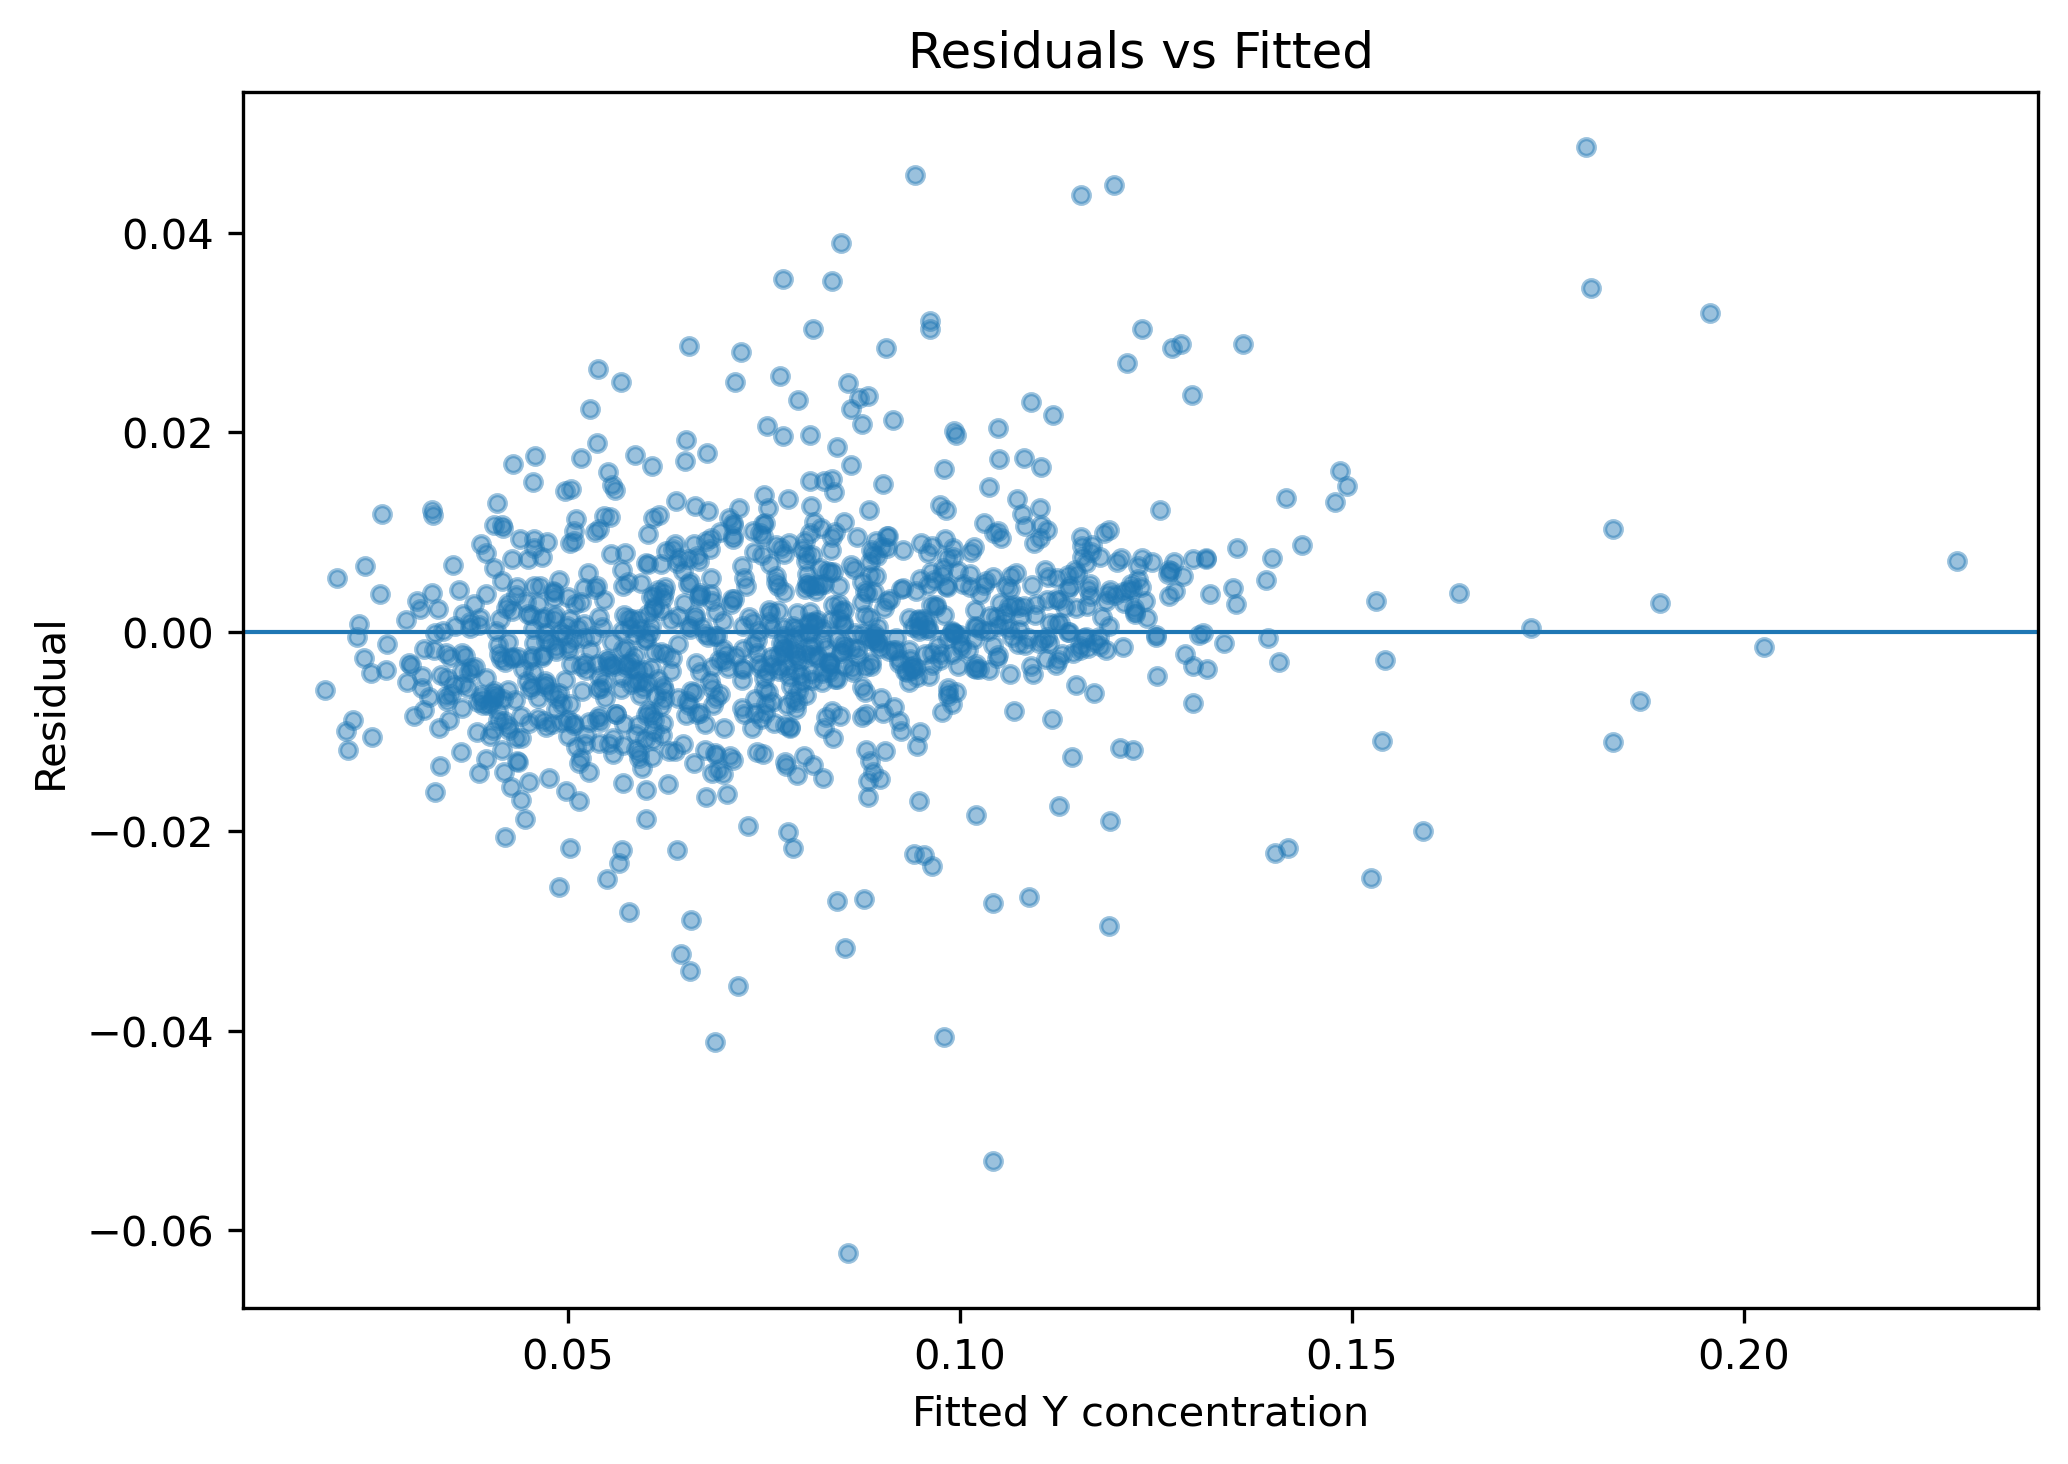
\includegraphics[width=\textwidth]{q1_residual_vs_fitted.png}
    \caption{残差与拟合值}
  \end{subfigure}
  \hfill
  \begin{subfigure}[t]{0.49\textwidth}
    \centering
    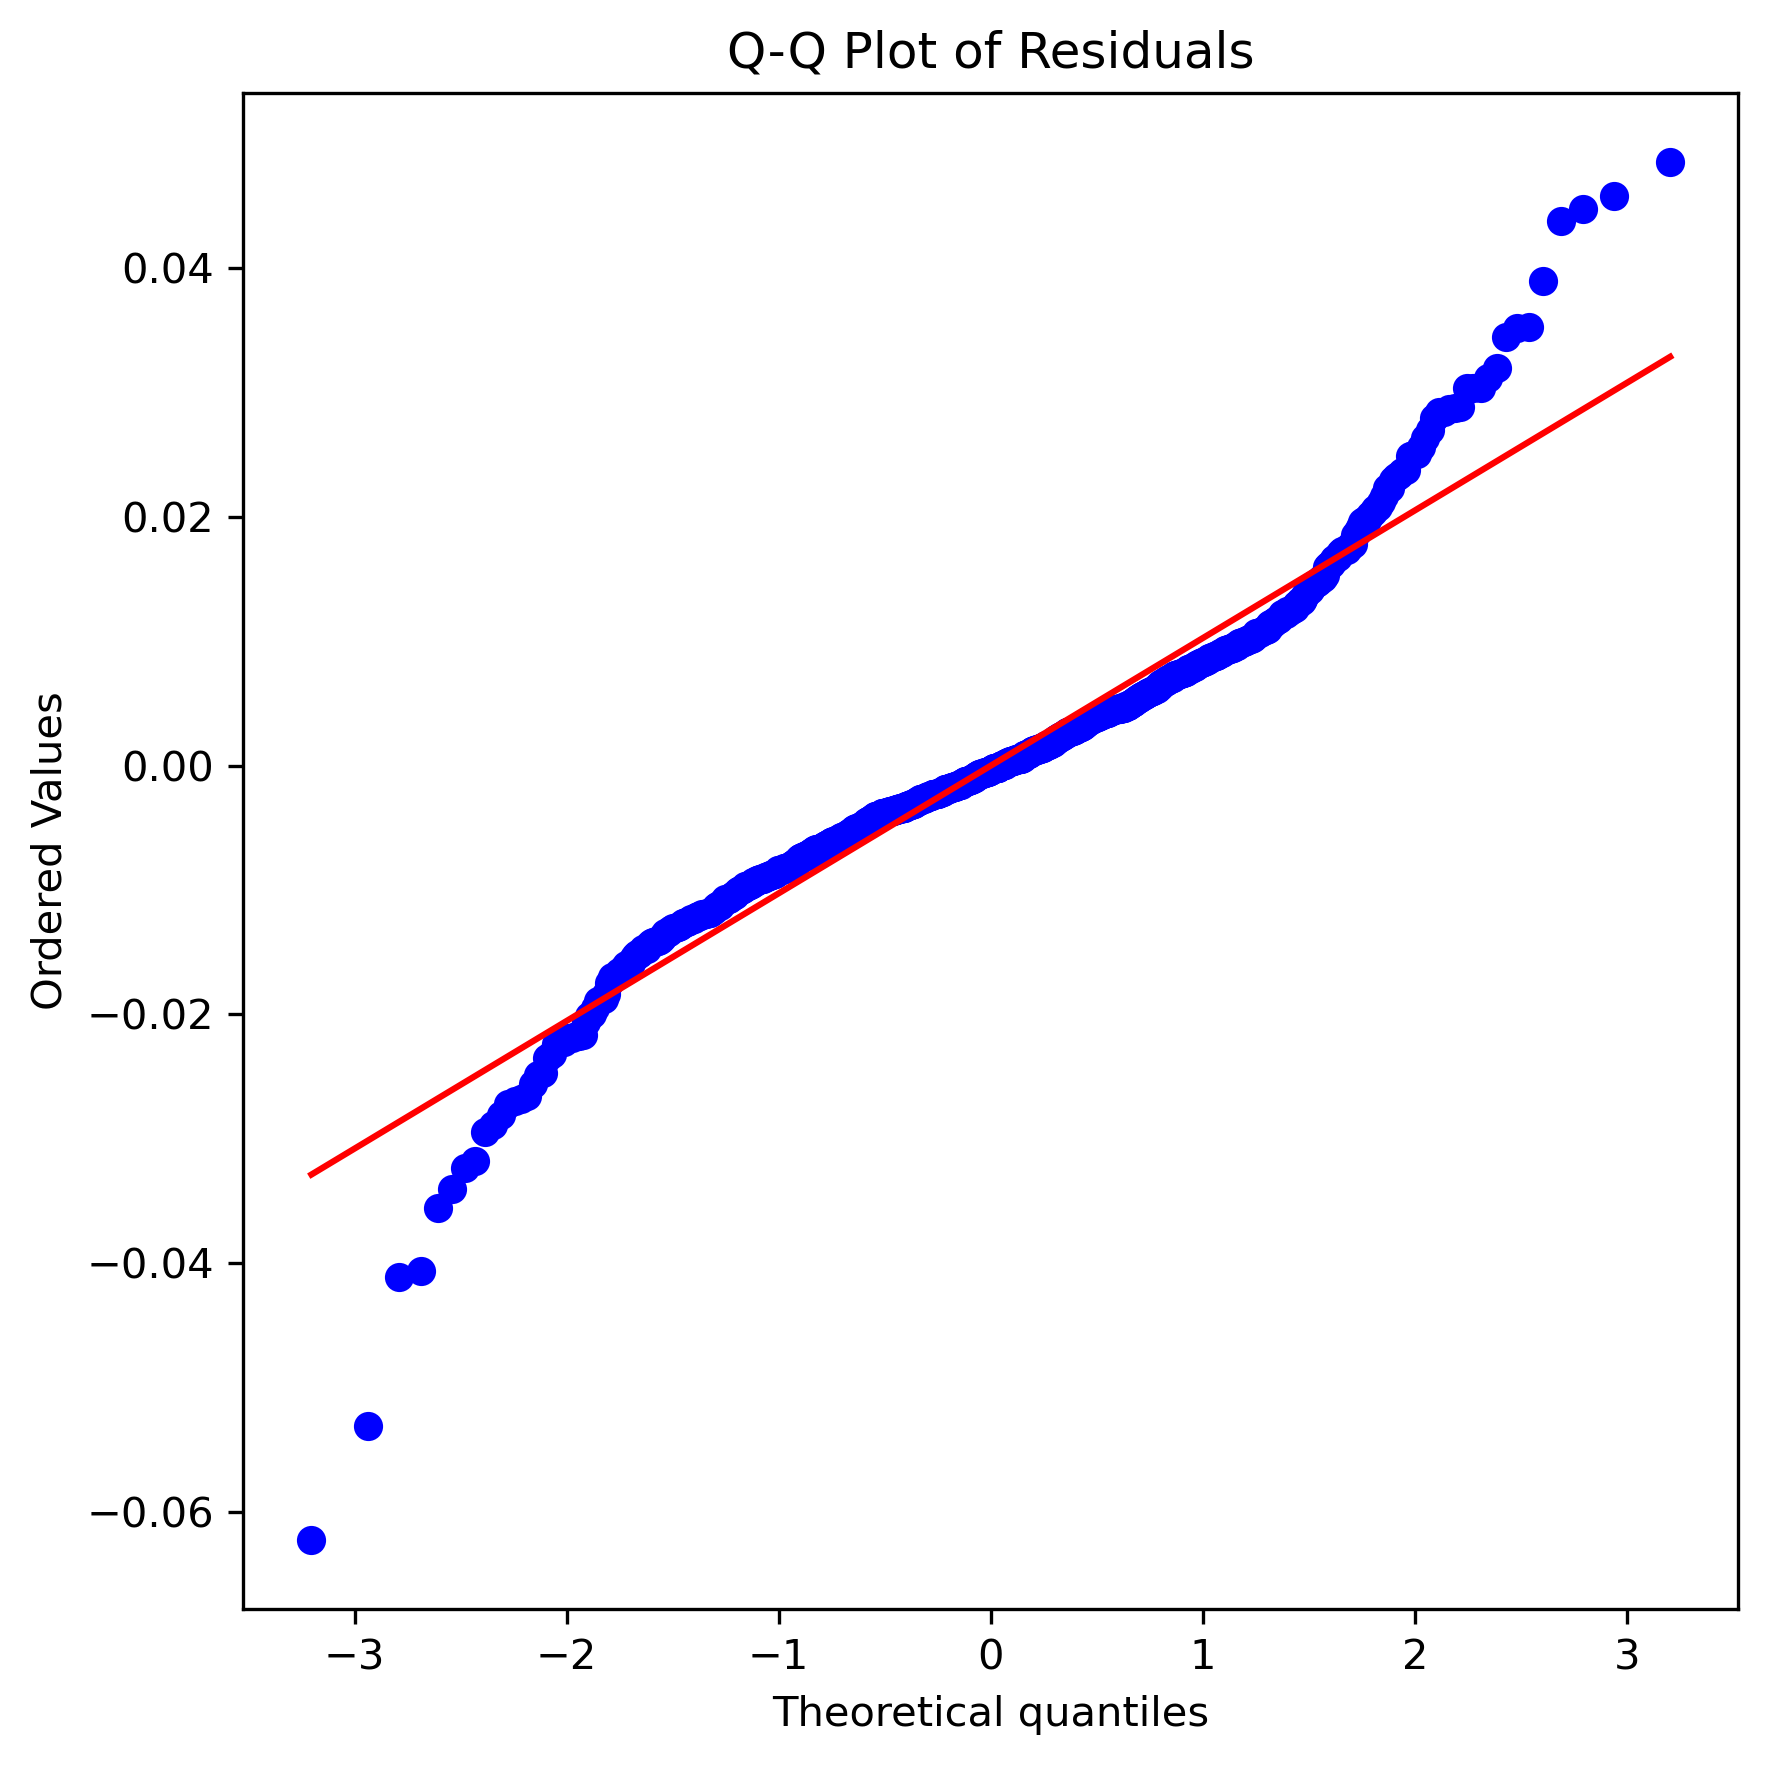
\includegraphics[width=\textwidth]{q1_residual_qq.png}
    \caption{残差Q--Q图}
  \end{subfigure}
  \caption{问题一线性混合效应模型诊断}
  \label{fig:q1-diagnostics}
\end{figure}

为检验同次采血取均值是否人为改变结论，使用1082条未聚合测序记录重新拟合同一模型。结果见表~\ref{tab:q1-sensitivity}，孕周、孕周平方和BMI的方向与显著性均保持不变，年龄在两种口径下均不显著，说明核心统计结论对聚合处理稳健。

\begin{table}[H]
  \centering
  \small
  \caption{聚合与未聚合数据的固定效应敏感性比较}
  \label{tab:q1-sensitivity}
  \begin{tabular}{lrrrr}
    \toprule
    变量 & 主模型系数 & 主模型$p$值 & 未聚合系数 & 未聚合$p$值 \\
    \midrule
    中心化孕周 & 0.003176 & $<0.001$ & 0.003197 & $<0.001$ \\
    中心化孕周平方 & 0.000264 & $<0.001$ & 0.000270 & $<0.001$ \\
    BMI & -0.001486 & 0.0046 & -0.001395 & 0.0070 \\
    年龄 & -0.000515 & 0.2908 & -0.000481 & 0.3238 \\
    \bottomrule
  \end{tabular}
\end{table}

40组同次采血重复测序的Y染色体浓度组内极差中位数为0.00884，95分位数为0.01780，最大值为0.02363。相较于题目使用的$4\%$阈值，这种测量波动不宜忽略，其分布见图~\ref{fig:q1-replicate-error}。该结果既支持Q1采用采血层面聚合，也为问题二的阈值误差扰动提供依据。

\begin{figure}[H]
  \centering
  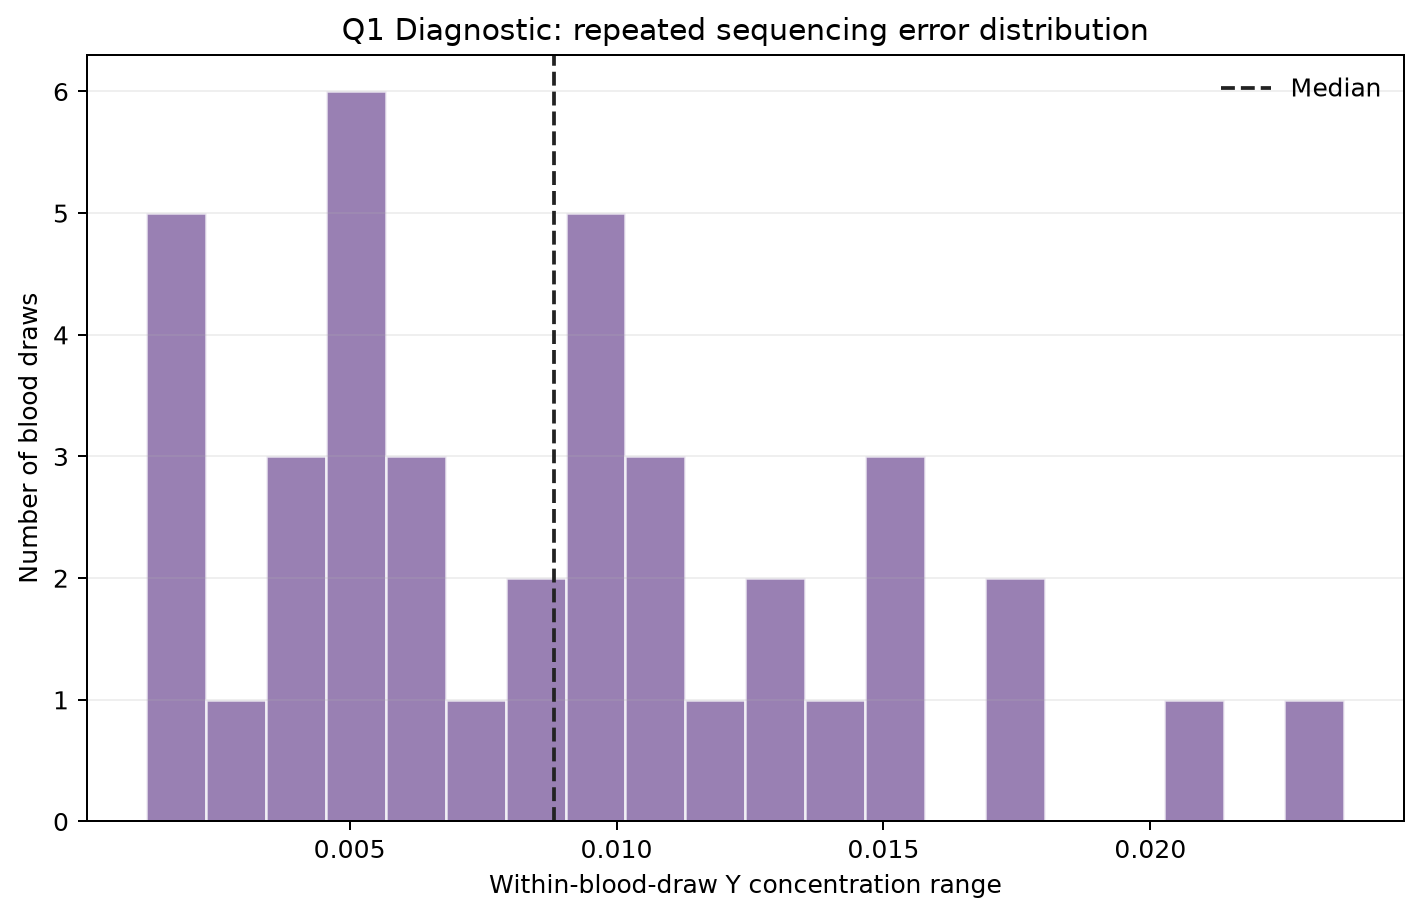
\includegraphics[width=0.82\textwidth]{q1_replicate_error.png}
  \caption{同次采血重复测序的Y染色体浓度极差分布}
  \label{fig:q1-replicate-error}
\end{figure}

\subsection{问题一结论及与问题二的衔接}

问题一识别出男胎Y染色体浓度随孕周呈显著非线性上升趋势，BMI对Y染色体浓度具有显著负向影响，而年龄在控制其他因素后未表现出显著独立效应；同时，孕妇之间存在明显的基础水平和孕周变化速度差异。由此，问题二应将连续浓度关系进一步转化为“达到$4\%$阈值的概率与时间”问题，以孕周和BMI建立达标概率模型，并在重复测序误差下寻找不同BMI人群的可靠检测时点。

\section{问题二的模型建立与求解}

\subsection{与问题一的联系及总体思路}

问题一用于识别孕周、BMI等指标与Y染色体浓度之间的关系；问题二进一步把这种关系转化为可执行的检测决策。其核心不再只是解释Y染色体浓度如何变化，而是回答“不同BMI孕妇在何时检测，既能保证足够的达标概率，又能尽量避免延迟发现风险”。

为此，本文采用“纵向达标概率建模—可靠性约束下的时点反演—CART自动分组—误差与稳定性检验”的四步框架。首先利用问题一统一得到的1021次采血记录建立达标概率模型；随后反演不同BMI水平达到目标可靠性的最早孕周；再利用一维CART将连续BMI压缩为若干可解释区间；最后使用Bootstrap和重复测序误差扰动检验结果稳定性。

\subsection{首次观测达标孕周的探索性分析}

先对260名曾观测到Y染色体浓度达标的孕妇，绘制基线BMI与首次观测达标孕周$T$的散点图，结果见图~\ref{fig:q2-bmi-week}。Spearman秩相关系数为$\rho=0.0878$，双侧检验$p=0.158$，表明二者仅呈极弱且不显著的正相关。

\begin{figure}[H]
  \centering
  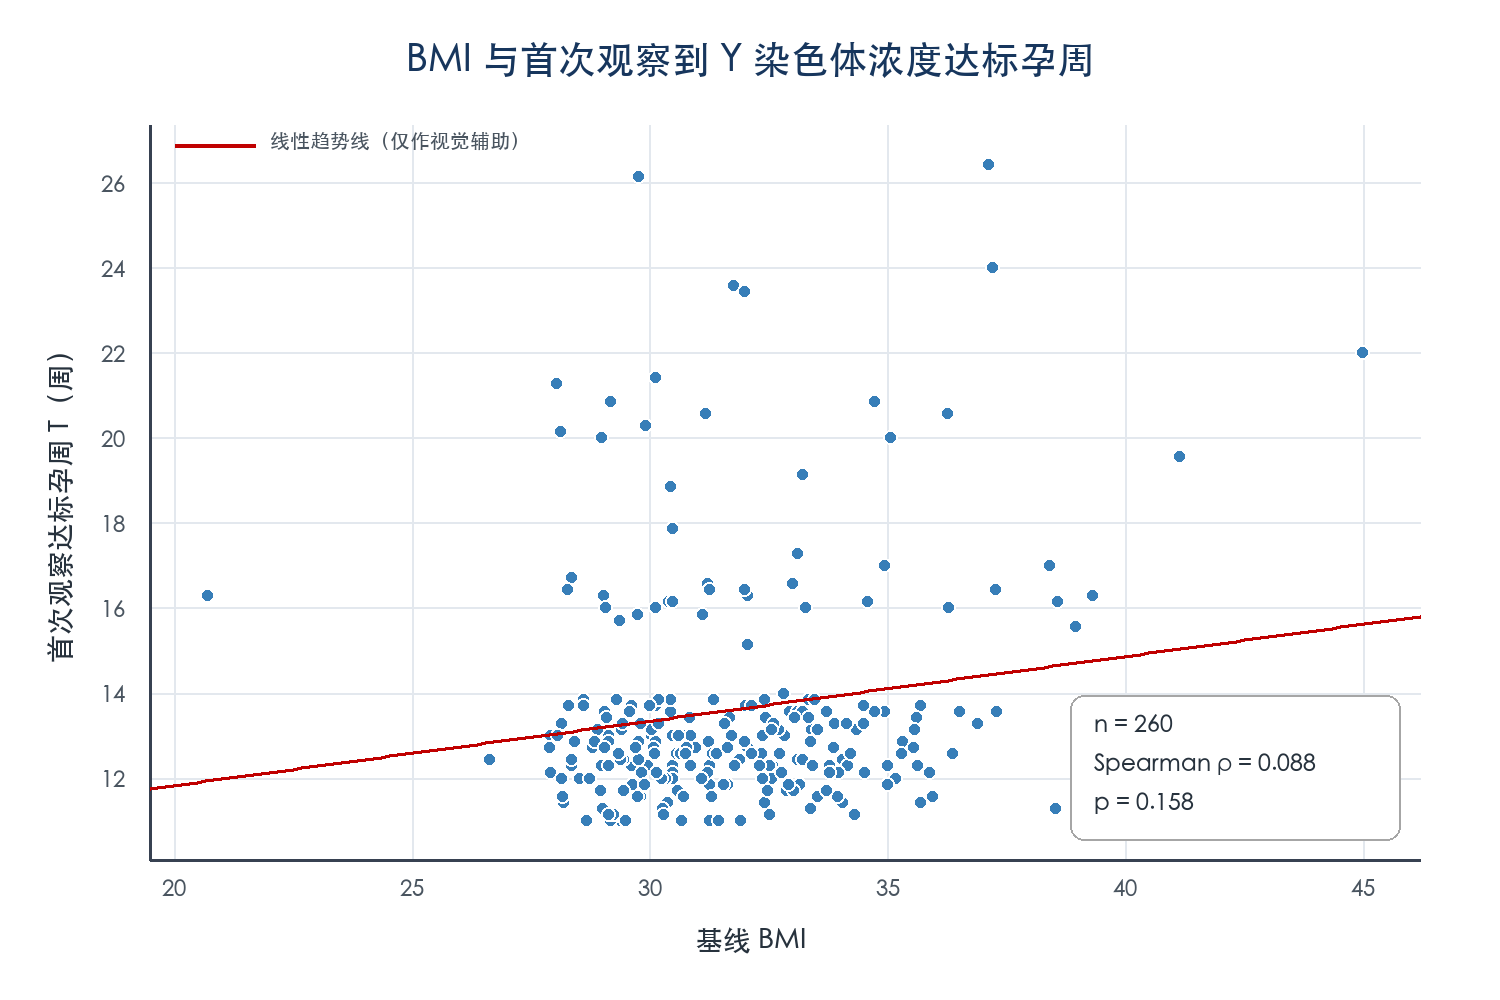
\includegraphics[width=0.92\textwidth]{q2_bmi_first_observed_week.png}
  \caption{基线BMI与首次观测Y染色体浓度达标孕周}
  \label{fig:q2-bmi-week}
\end{figure}

上述弱相关不能直接解释为BMI没有作用。由第~\ref{eq:q2-status}式可知，达标时间的观测依赖于实际采样安排；特别是首次检测已经达标的217名孕妇，其真实达标时刻只能确定为早于首次检测。若直接对首次观测达标孕周进行普通回归或CART分组，会把“何时接受检测”与“何时生理达标”混为一谈。因此，本文不把图~\ref{fig:q2-bmi-week}中的$T$作为主模型的连续响应变量，而改用每名孕妇的全部纵向检测记录建立达标概率模型。

\subsection{纵向达标概率模型}

\subsubsection{模型设定}

设$W_{ij}$为第$i$名孕妇第$j$次独立采血时的孕周，$B_i$为其基线BMI，$D_{ij}$为第~\ref{eq:q2-status}式定义的达标状态。记

\begin{equation}
  p_{ij}=P\!\left(D_{ij}=1\mid W_{ij},B_i\right).
  \label{eq:q2-probability}
\end{equation}

候选模型包括线性Logistic回归、含二次项与交互项的Logistic回归、样条Logistic回归和梯度提升树，并设置仅使用总体达标率的常数模型作为基准。线性Logistic模型写为

\begin{equation}
  \operatorname{logit}(p_{ij})
  =\beta_0+\beta_1W_{ij}+\beta_2B_i.
  \label{eq:q2-logistic}
\end{equation}

由于各孕妇的检测次数不同，若给每条记录相同权重，检测次数较多的孕妇会对参数估计产生过大影响。因此，将第$i$名孕妇全部记录的总权重设为1，每条记录权重取其检测次数的倒数。

\subsubsection{分组交叉验证与模型选择}

为防止同一孕妇的多次记录同时出现在训练集和验证集中，采用以孕妇代码为分组单位的五折交叉验证。模型选择以LogLoss为主要指标，Brier得分和AUC为辅助指标；LogLoss和Brier越小，说明概率预测越准确，AUC越大，说明区分达标与未达标记录的能力越强。相关方法可参考Logistic回归与统计学习理论\cite{hosmer2013applied,hastie2009elements}。

\begin{table}[H]
  \centering
  \caption{候选达标概率模型的分组五折交叉验证结果}
  \label{tab:q2-model-cv}
  \begin{tabular}{ccccc}
    \toprule
    模型 & LogLoss & 标准误 & Brier & AUC \\
    \midrule
    二次交互Logistic & 0.3693 & 0.0254 & 0.1069 & 0.5854 \\
    线性Logistic & 0.3702 & 0.0252 & 0.1071 & 0.5862 \\
    样条Logistic & 0.3721 & 0.0269 & 0.1076 & 0.6001 \\
    梯度提升树 & 0.3751 & 0.0342 & 0.1086 & 0.6310 \\
    基准常数模型 & 0.3783 & 0.0293 & 0.1095 & 0.5000 \\
    \bottomrule
  \end{tabular}
\end{table}

\begin{figure}[H]
  \centering
  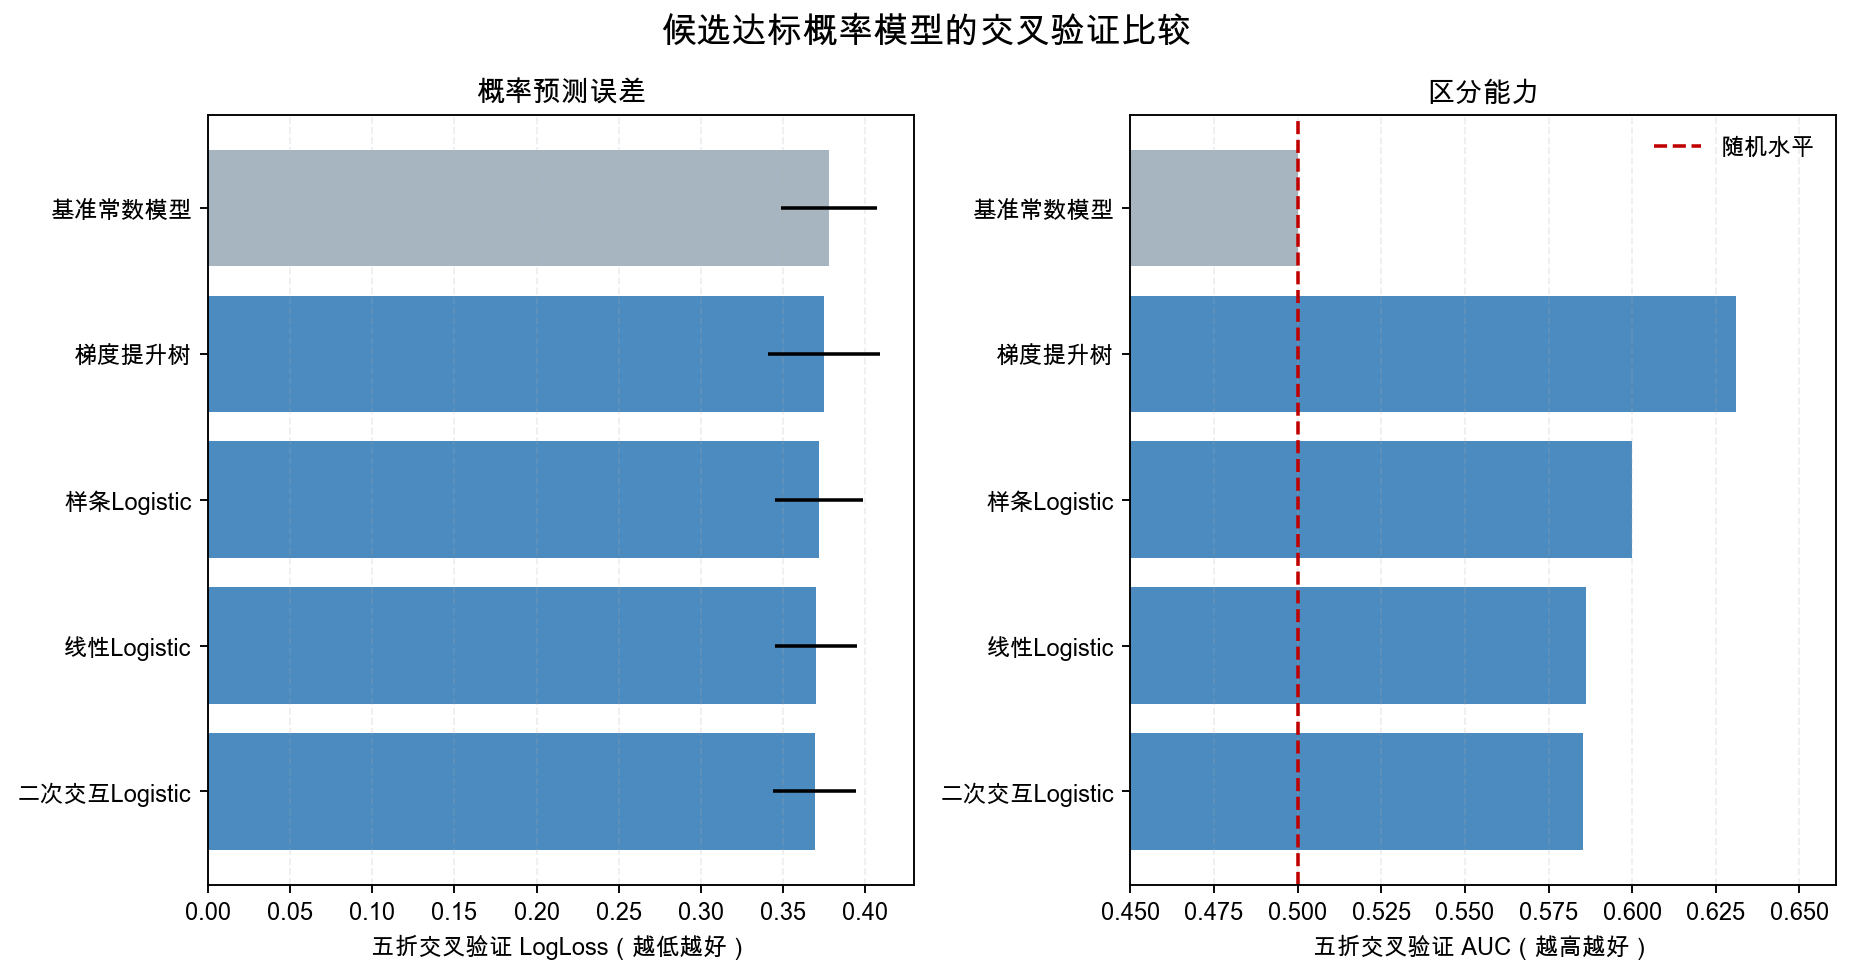
\includegraphics[width=0.96\textwidth]{q2_model_comparison.png}
  \caption{候选达标概率模型的交叉验证比较}
  \label{fig:q2-model-comparison}
\end{figure}

由表~\ref{tab:q2-model-cv}和图~\ref{fig:q2-model-comparison}可见，二次交互Logistic取得最低LogLoss，但其与线性Logistic的差值仅为0.0009，远小于相应交叉验证标准误0.0254。依据一标准误差规则，在预测误差没有显著恶化的情况下优先选择结构更简单的线性Logistic模型。梯度提升树虽然AUC相对较高，但LogLoss和Brier均较差，说明其概率校准能力不足，不适合作为本题时点反演的主模型。

将线性Logistic模型系数换算回原始量纲，得到

\begin{equation}
  \operatorname{logit}(p)
  =5.2836+0.0507W-0.1300B.
  \label{eq:q2-final-logistic}
\end{equation}

孕周系数为正、BMI系数为负，表示在控制另一变量后，孕周增加有利于Y染色体浓度达标，而BMI升高会降低同一孕周下的达标概率。不过，最终模型AUC仅为0.5862，说明只使用BMI和孕周时个体区分能力有限。因此，本文将该模型用于群体检测时点决策，不将其解释为高精度个体诊断模型。

\subsection{可靠性约束下的最佳检测时点}

题目要求同时兼顾检测准确性和尽早发现风险。本文采用词典序决策准则：首先满足预设的达标可靠性，在满足可靠性的可行孕周中选择最早时点。为符合群体达标概率一般不随孕周下降的规律，对预测概率曲线施加累积最大值约束。定义给定BMI下达到$90\%$预测达标概率的最早孕周为

\begin{equation}
  t_{0.90}(B)
  =\min\left\{w:P(Y\geq0.04\mid B,w)\geq0.90\right\},
  \quad 10\leq w\leq25.
  \label{eq:q2-target-week}
\end{equation}

对第$g$个BMI组，令$\bar p_g(w)$为组内孕妇在孕周$w$的平均预测达标概率，则推荐时点为

\begin{equation}
  t_g^{*}=\min\left\{w:\bar p_g(w)\geq q_g\right\}.
  \label{eq:q2-group-week}
\end{equation}

通常取$q_g=0.90$。若某组在25周内仍不能达到$90\%$，则将可行阈值降为$85\%$，在达到该阈值的最早孕周先行检测，并对未达标样本安排复测。该规则避免为了追求小幅准确率提升而把检测过度推迟至治疗窗口更加紧张的阶段。

\subsection{基于CART的BMI自动分组}

以基线BMI为输入、模型反演得到的$t_{0.90}$为输出，建立一维CART回归树\cite{breiman1984cart}。CART通过选择BMI切点，使各叶节点内预测达标时点的离差平方和最小：

\begin{equation}
  \min_{G_1,\ldots,G_K}
  \sum_{g=1}^{K}\sum_{i\in G_g}
  \left(t_i-\bar t_g\right)^2.
  \label{eq:q2-cart-objective}
\end{equation}

为保证分组具有基本样本量，规定每个叶节点至少包含22名孕妇，并比较3至5个叶节点的方案。相应五折交叉验证MAE分别为1.354、0.830和0.753周；根据一标准误差规则，5组方案仍是唯一满足阈值的方案，故最终选择5个BMI组。模型确定的切点为28.63、29.59、31.30和32.70，分组结果如图~\ref{fig:q2-cart-groups}所示。

\begin{figure}[H]
  \centering
  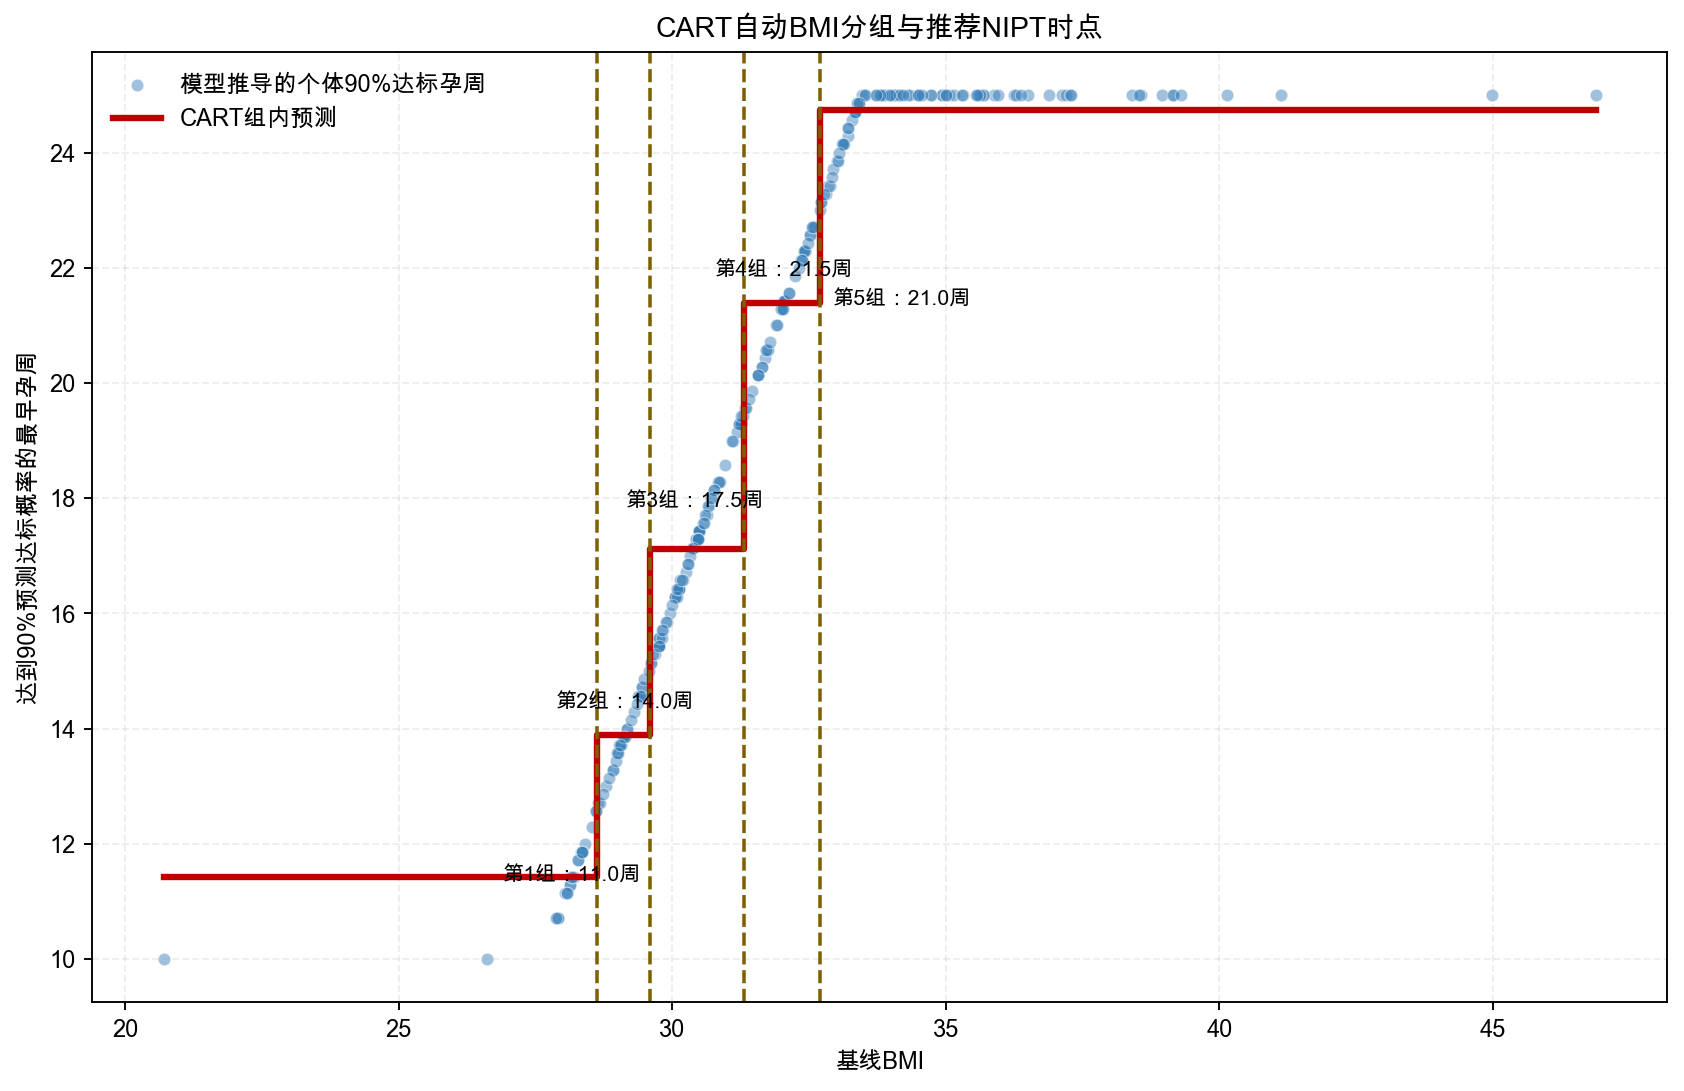
\includegraphics[width=0.96\textwidth]{q2_bmi_groups.png}
  \caption{CART自动BMI分组与推荐NIPT时点}
  \label{fig:q2-cart-groups}
\end{figure}

\begin{table}[H]
  \centering
  \small
  \caption{BMI分组、推荐检测时点及预测可靠性}
  \label{tab:q2-group-result}
  \begin{tabularx}{\textwidth}{c>{\centering\arraybackslash}Xcccc}
    \toprule
    组别 & BMI区间 & 人数 & 推荐孕周 & 平均达标率 & 检测策略 \\
    \midrule
    1 & $B<28.63$ & 23 & 11.0 & 90.1\% & 满足90\%约束 \\
    2 & $28.63\leq B<29.59$ & 35 & 14.0 & 90.1\% & 满足90\%约束 \\
    3 & $29.59\leq B<31.30$ & 76 & 17.5 & 90.2\% & 满足90\%约束 \\
    4 & $31.30\leq B<32.70$ & 43 & 21.5 & 90.1\% & 满足90\%约束 \\
    5 & $B\geq32.70$ & 90 & 21.0 & 85.2\% & 初检后安排复测 \\
    \bottomrule
  \end{tabularx}
\end{table}

由表~\ref{tab:q2-group-result}可知，前四组均选择达到$90\%$平均达标概率的最早时点。第五组在25周内仍无法达到$90\%$，因此按照第~\ref{eq:q2-group-week}式的备用规则，在21.0周达到$85\%$时先进行初检，并对未达标者尽快复测。由此可见，第五组推荐时点略早于第四组并非模型认为高BMI孕妇更早达标，而是两组采用了不同的可靠性约束；这种处理体现了对延迟风险的控制。

不同BMI组的达标概率曲线如图~\ref{fig:q2-probability-curves}所示。总体上，BMI越高，同一孕周下的预测达标概率越低，达到$90\%$可靠性所需的时间越晚。最高BMI组在25周内仍未达到$90\%$水平，也说明对其采用“较早初检加复测”比单纯延迟更为合理。

\begin{figure}[H]
  \centering
  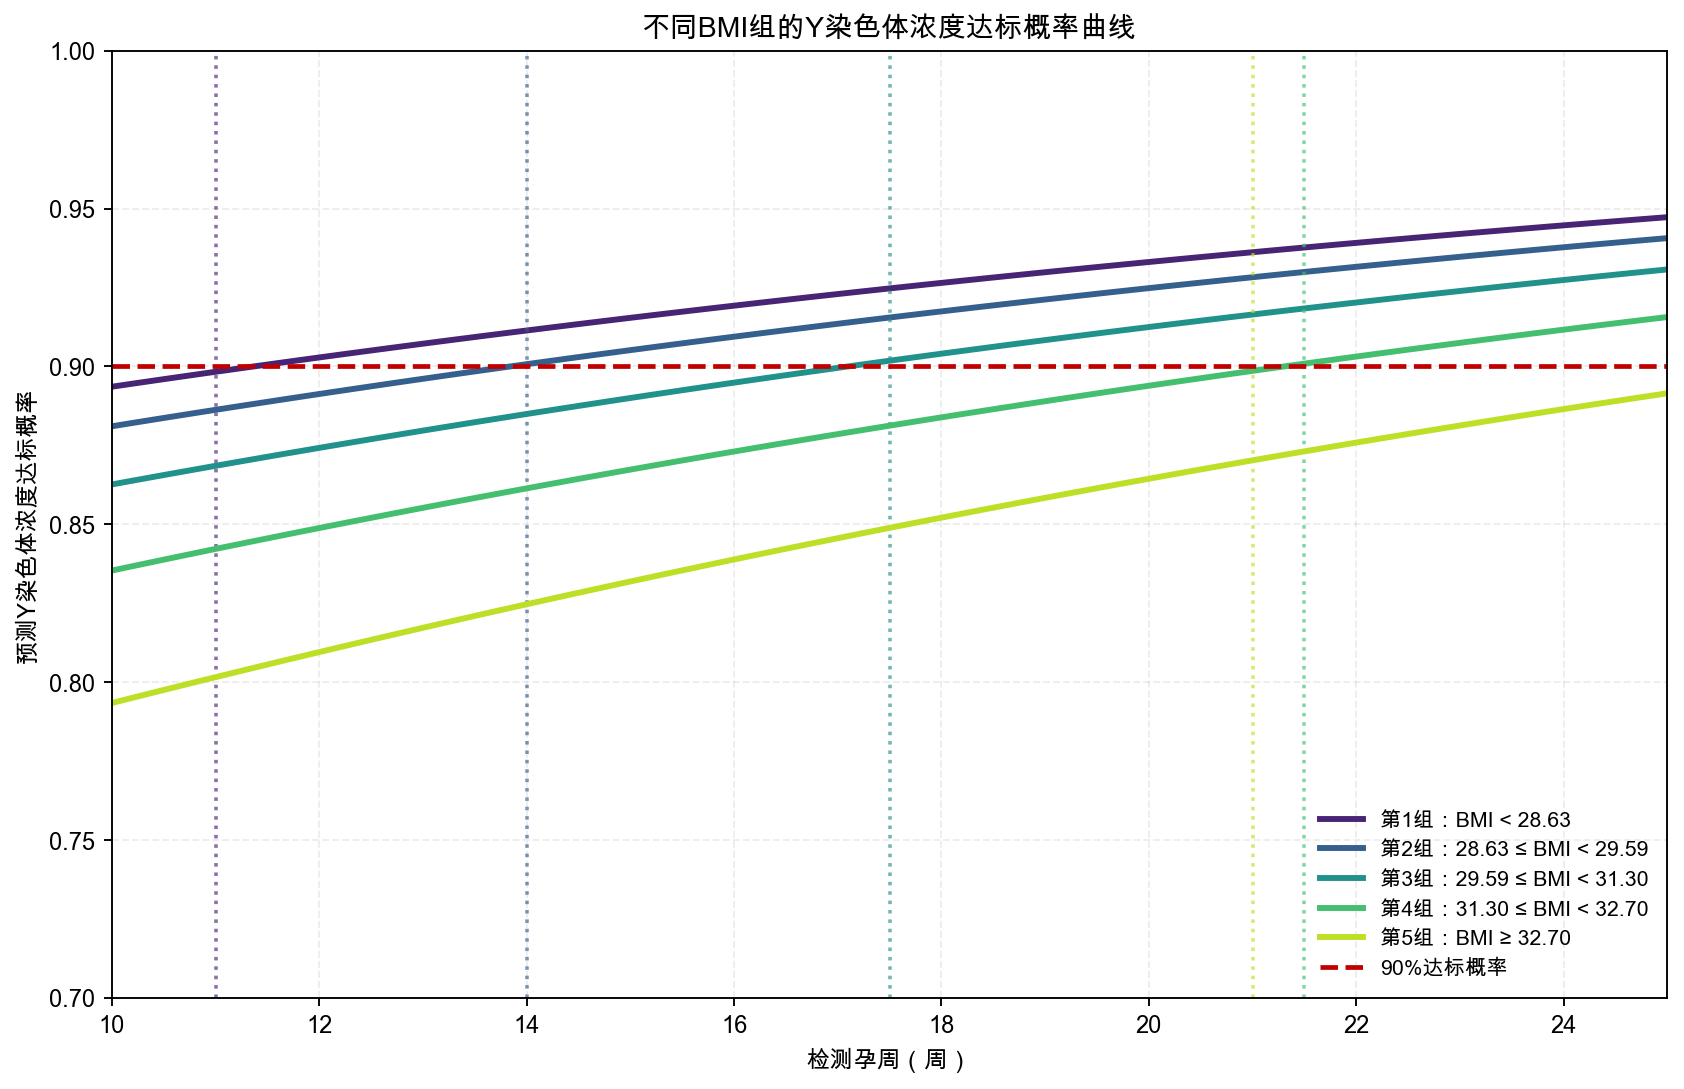
\includegraphics[width=0.96\textwidth]{q2_probability_curves.png}
  \caption{不同BMI组的Y染色体浓度预测达标概率曲线}
  \label{fig:q2-probability-curves}
\end{figure}

\subsection{分组稳定性与检测误差分析}

\subsubsection{BMI切点的Bootstrap稳定性}

对267名孕妇进行300次Bootstrap有放回抽样，每次重新拟合5叶节点CART并记录切点，结果见表~\ref{tab:q2-bootstrap}。

\begin{table}[H]
  \centering
  \caption{300次Bootstrap下BMI切点的稳定性}
  \label{tab:q2-bootstrap}
  \begin{tabular}{cccc}
    \toprule
    切点 & 原始值 & Bootstrap中位数 & 95\%区间 \\
    \midrule
    1 & 28.63 & 28.98 & $[28.51,29.65]$ \\
    2 & 29.59 & 29.79 & $[29.34,31.00]$ \\
    3 & 31.30 & 31.30 & $[31.02,31.84]$ \\
    4 & 32.70 & 32.66 & $[32.50,32.84]$ \\
    \bottomrule
  \end{tabular}
\end{table}

第四切点的区间较窄，稳定性相对较好；前三个切点存在不同程度漂移。由于第一组样本量仅为23，表中保留两位小数主要用于模型复现，实际应用时更适合按照约0.5个BMI单位进行近似解释，不宜将切点视为绝对精确的临床边界。

\subsubsection{Y染色体浓度测量误差}

对于40组同次采血重复测序，设组内最大值与最小值之差为$\Delta$。在把该极差近似视为两次独立测量之差的条件下，若单次测量误差独立同分布且方差为$\sigma^2$，则

\begin{equation}
  \operatorname{Var}(\Delta)=2\sigma^2.
  \label{eq:q2-error-variance}
\end{equation}

据此估计单次Y染色体浓度测量误差标准差为$\sigma=0.007378$，即0.738个百分点。随后对每条Y染色体浓度加入$N(0,\sigma^2)$扰动，重复200次重新判断$4\%$阈值、拟合概率模型并计算推荐时点。平均约有5.0\%的采血记录在扰动后跨越$4\%$阈值。

\begin{table}[H]
  \centering
  \caption{200次测量误差扰动下推荐时点的稳定性}
  \label{tab:q2-error-result}
  \begin{tabular}{cccc}
    \toprule
    组别 & 原始推荐孕周 & 扰动中位数 & 95\%扰动区间 \\
    \midrule
    1 & 11.0 & 13.0 & $[10.0,17.5]$ \\
    2 & 14.0 & 16.5 & $[10.5,20.0]$ \\
    3 & 17.5 & 20.0 & $[10.0,24.5]$ \\
    4 & 21.5 & 22.0 & $[10.0,25.0]$ \\
    5 & 21.0 & 22.5 & $[19.5,25.0]$ \\
    \bottomrule
  \end{tabular}
\end{table}

\begin{figure}[H]
  \centering
  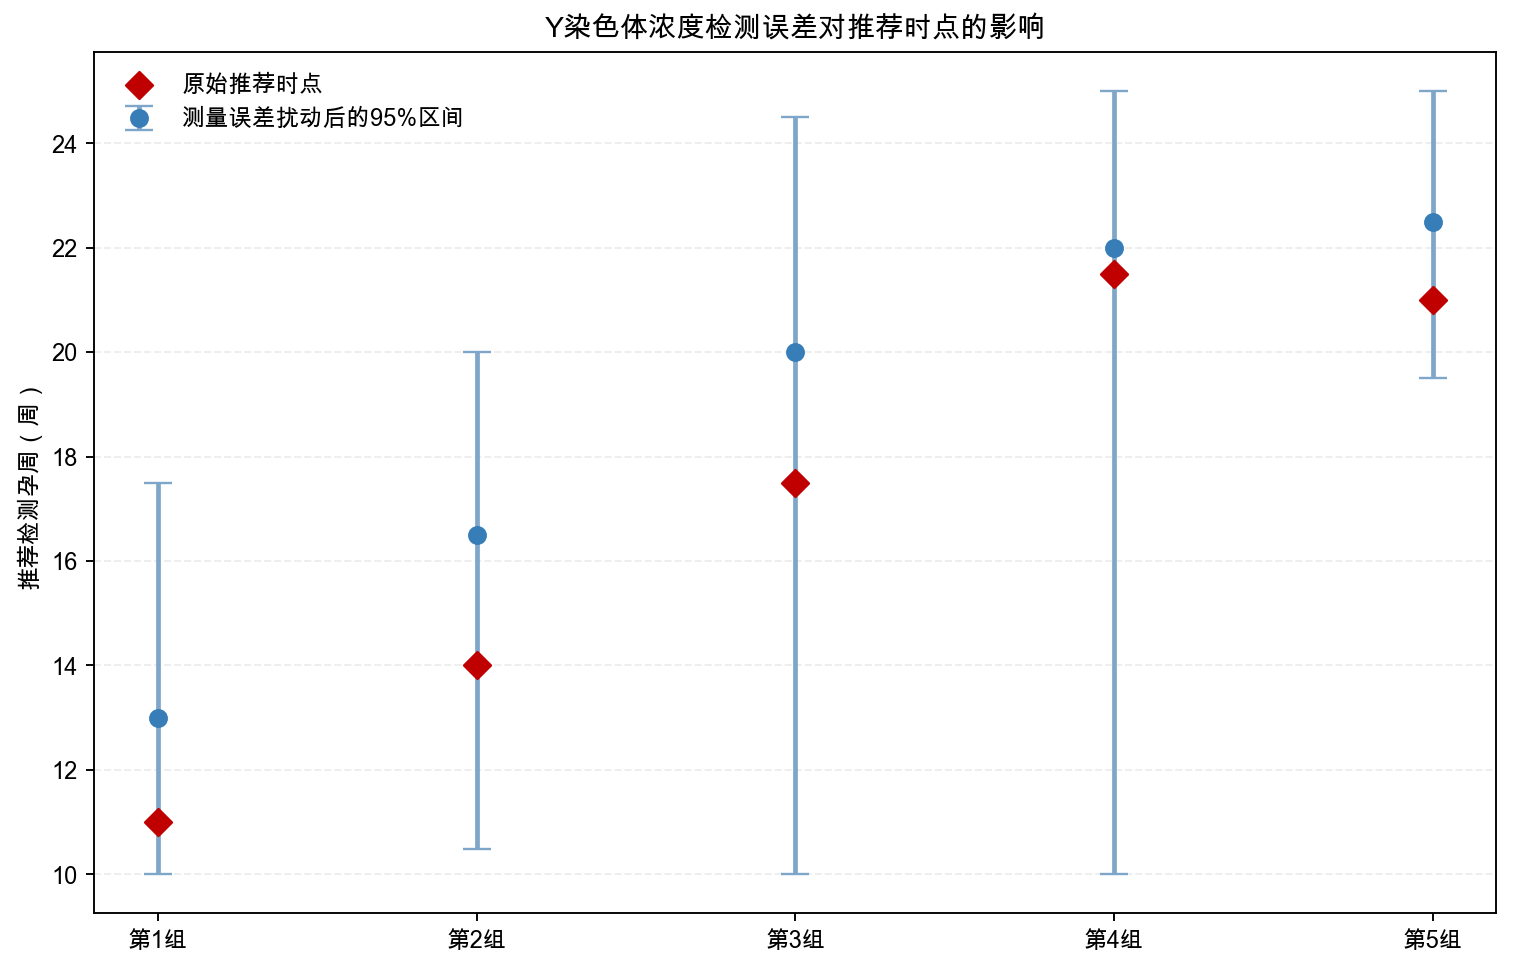
\includegraphics[width=0.90\textwidth]{q2_error_sensitivity.png}
  \caption{Y染色体浓度检测误差对推荐时点的影响}
  \label{fig:q2-error-sensitivity}
\end{figure}

由表~\ref{tab:q2-error-result}和图~\ref{fig:q2-error-sensitivity}可知，第五组推荐时点中位数为22.5周，与原方案方向基本一致；各组尤其是中间BMI组的扰动区间较宽，表明接近$4\%$阈值的测量误差可能明显改变推荐时点。因此，表~\ref{tab:q2-group-result}给出的时点应理解为群体层面的基准建议，对于临界BMI或临界Y浓度样本，应结合复测进行个体化判断。

\subsection{问题二结论与模型评价}

本文最终将男胎孕妇划分为$B<28.63$、$[28.63,29.59)$、$[29.59,31.30)$、$[31.30,32.70)$和$B\geq32.70$五组，推荐初次NIPT检测时点依次为11.0、14.0、17.5、21.5和21.0周。其中，最高BMI组由于在25周内不能达到$90\%$预测达标概率，采用21.0周达到$85\%$后先行检测并安排复测的策略。

该方法利用全部纵向采血记录，避免把首次观测达标孕周误认为精确生理达标时间；按孕妇代码分组的交叉验证减少了数据泄漏；一标准误差规则、最小叶节点约束和Bootstrap共同限制模型复杂度；误差扰动进一步量化了$4\%$阈值附近的不确定性。其局限在于样本以高BMI孕妇为主，低BMI组样本量较少，且最终Logistic模型AUC仅为0.5862。因此，本问结果适合作为相似人群的群体检测时点参考，问题三还需加入年龄、身高、体重和测序质量等因素提高个体化能力。

% 问题三由负责同学完成后，将正文写入本文件。
% 建议结构：多因素达标概率模型、BMI分组与时点优化、误差分析。

% 问题四由负责同学完成后，将正文写入本文件。
% 建议结构：标签构造、特征处理、分类模型、分组验证和评价指标。


% ========================= 参考文献 =========================
\bibliographystyle{unsrt}
\bibliography{references}

% =========================== 附录 ===========================
\newpage
\begin{appendices}

\section{支撑材料文件说明}
为避免整段程序挤占论文正文篇幅，源代码、清洗数据和程序结果均作为独立支撑材料随论文一并保存：
\begin{itemize}
  \item 问题一核心程序：\path{code/q1_final_model.py}；
  \item 问题一程序结果：\path{results/q1/}；
  \item 问题一正文插图：\path{figures/q1/}；
  \item 问题二核心程序：\path{code/q2_optimal_timing.py}；
  \item 问题二清洗数据：\path{data/processed/q2_male_cleaned.xlsx}；
  \item 问题二程序结果：\path{results/q2/}；
  \item 问题二正文插图：\path{figures/q2/}。
\end{itemize}
正式提交时，应按照比赛当年的支撑材料要求单独提交程序和数据文件，不在论文正文中粘贴完整代码。

\end{appendices}

\end{document}
